%!TEX root = ../main.tex
%-------------------------------------------------------------------------------
%                            	BAB IV
%               		IMPLEMENTASI DAN PENGUJIAN
%-------------------------------------------------------------------------------

\chapter{HASIL DAN PEMBAHASAN}

\section{Implementasi}

Terdapat perubahan pada \emph{interface} yang telah dibuat pada gambar 3.2. Perubahan serta fungsionalitas dari \emph{method} pada interface akan 
dijelaskan pada sub bab implementasi dibawah. Selain itu, terdapat perbedaan pada bahasa pemrograman yang di jelaskan pada gambar 3.2, bahasa pemrograman
yang digunakan dalam penelitian ini adalah bahasa \emph{low-level} bernama rust. Versi bahasa rust yang digunakan pada saat pengembangan adalah
rust dengan versi 1.84.1, namun untuk menjalankan hasil akhir dari \emph{database engine} ini, tidak perlu menginstall bahasa rust karena hasil akhir atau hasil build
dari bahasa rust merupakan \emph{file} \emph{bin} yang dapat langsung dijalankan.

\subsection{Bahasa Pemrograman Rust}
Rust merupakan salah satu bahasa pemrograman yang mempunyai tingkat kecepatan yang tinggi. Berdasarkan web resmi dari dokumentasi rust,
rust memiliki performa yang baik, ketahanan yang baik dan produktivitas yang baik (dokumentasi yang lengkap). Rust dapat digunakkan pada
teknologi \emph{low-level} seperti embedding system, web assembly, pembuatan command line dan lainnya. Berdasarkan paper \emph{Towards Understanding 
the Runtime Performance of Rust} \cite{yuchen2022}, kecepatan performa rust tidak jauh berbeda dengan bahasa pemrograman C. Dengan begitu rust 
menjadi salah satu bahasa tercepat untuk saat ini. Rust bukanlah bahasa pemrograman yang mengadopsi Object Oriented Programming sehingga 
tidak memiliki class. Namun terdapat alternatif dalam penggunaan \emph{class} yaitu struct. Agar penulisan lebih jelas dan mudah dipahami, istilah
class akan digunakan daripada istilah struct.

Dengan membuat menggunakan bahasa rust, hasil akhir dari pengembangan ini akan dilakukan sebuah proses yang bernama \emph{build}. Dari proses \emph{build} ini,
database akan berjalan. Jika sudah dalam bentuk hasil \emph{build}, maka sudah tidak perlu memasang bahasa rust pada komputer yang dituju karena hasil dari \emph{build}
merupakan \emph{file} yang dapat dijalankan secara langsung.

\subsection{Struktur Folder}
Struktur folder yang digunakan merupakan dasar struktur \emph{folder} dari rust. Dalam \emph{folder} src terdapat \emph{folder} \emph{database} yang berisi \emph{class} dan \emph{method}
yang akan digunakan dalam menjalankan \emph{database engine}. Terdapat 1 \emph{file} bernama playground.js hanya sebagai penyimpanan code saat pengembangan. 
dan tidak digunakan pada \emph{database engine}. Terdapat 3 \emph{folder} tambahan di bagian \emph{root} \emph{folder}, yaitu client-test (untuk menyimpan pengujian client),
schema (menyimpan \emph{file} \emph{database}) dan \emph{index} (untuk menyimpan \emph{index} yang terdapat pada database). Lalu di bagian \emph{root} \emph{folder} juga terdapat \emph{folder} test-data, dalam \emph{folder} ini
berguna untuk menyimpan data-data yang berguna untuk testing dan dokumentasi. Terdapat dapat beberapa \emph{file} seperti article.json, crawling.json, dan crawl\_information.json 
untuk menampung data pengujian sementara dan test.js yang hanya digunakan untuk membantu penulisan (Untuk memanfaatkan \emph{extension prettier} untuk
mempercantik dokumentasi hasil data, seperti pada gambar 4.19). Berikut adalah struktur \emph{folder} dari \emph{database engine}:

\begin{figure}[H]
  \centering{}
	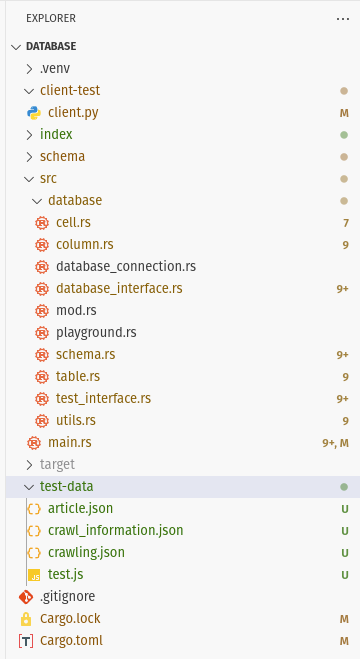
\includegraphics[width=0.3\textwidth]{gambar/bab4/struktur-folder.png}
  \caption{Struktur Folder}
\end{figure}


\subsection{Schema}
Class Schema merupakan \emph{class} induk pada \emph{database engine} yang dibuat. \emph{Class} ini menampung bagian penyimpanan data dan sebagai portal bagi pengolahan
data yang terjadi pada \emph{database engine}. \emph{Class} Schema ini akan merepresentasikan satu entitas \emph{database}. Berikut adalah \emph{class} diagram dari \emph{class} Schema.
\begin{figure}[H]
  \centering{}
	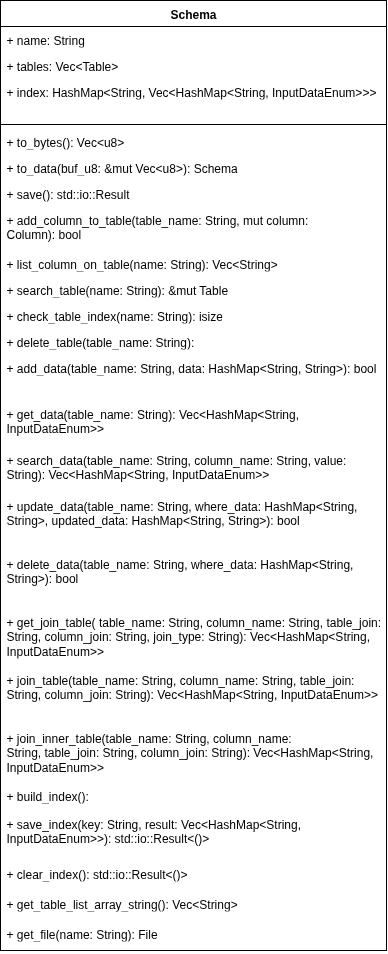
\includegraphics[width=0.3\textwidth]{gambar/bab4/Schema}
  \caption{Class Diagram Schema}
\end{figure}

Atribut dan \emph{method} yang tertulis pada \emph{class} diagram berguna untuk fitur yang ada di \emph{database} dan juga berguna saat pengembangan \emph{database engine}.
Terdapat 3 attribut pada \emph{class} Schema, yaitu:
\begin{enumerate}
	\item name \\
	Berguna untuk menyimpan nama dari \emph{database} dalam bentuk tipe data string.

	\item tables \\
	Attribut ini berguna untuk menyimpan list tabel yang ada pada \emph{database} atau schema yang dibuat. Tipe data atribut ini adalah Vector berisi \emph{class} table, yang akan 
  dijelaskan pada pembahasan \emph{class} berikutnya. 

	\item index  \\
	Atribut ini berguna untuk menyimpan \emph{index} yang ada pada instance schema yang dibuat. Tipe data dari atribut ini adalah HashMap, dan berisi
  struktur data yang cukup kompleks atau dalam. Hasmap pada atribut index ini memiliki key dengan tipe String, dan value sebuah vector. Vector didalamnya
  berisi beberapa HashMap yang nanti digunakan sebagai baris data yang telah disimpan. Lalu HashMap terdalam ini mempunyai key String dengan Value \emph{class} InputDataEnum.
			
\end{enumerate}

Untuk menggunakan dan mengolah data-data yang ada di dalam atribut, dibutuhkan method-method yang sudah dibuat dalam \emph{class} Schema. Terdapat 21 \emph{method} yang dapat digunakan, yaitu:

\begin{enumerate}
	\item to\_bytes \\
  \emph{Method} ini berguna untuk mengubah data yang telah disimpan pada atribut tabel. \emph{Method} ini mengembalikan sebuah vector yang berisi u8. Tipe u8 ini yang akan mempresentasikan 
  \emph{bytes} dan disimpan dalam \emph{filesystem}. Penyimpanan \emph{bytes} dalam vector memiliki urutan yang harus diperhatikan dan tidak boleh salah. Karena jika salah dapat menyebabkan data gagal
  diambil. Berikut adalah ilustrasi urutan dari penyimpanan \emph{byte} untuk \emph{class} Schema.

  \begin{figure}[H]
	\centering{}
		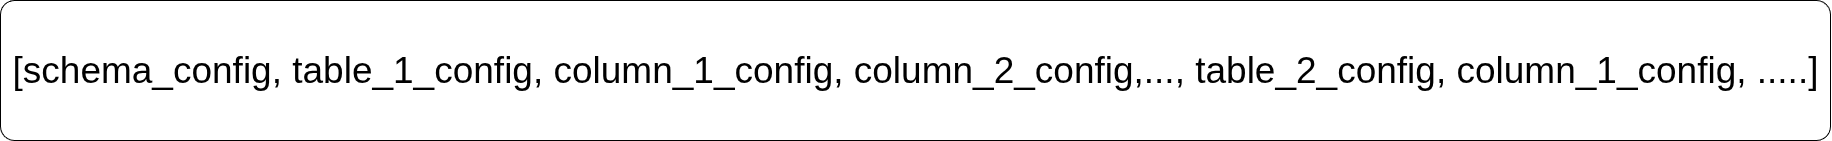
\includegraphics[width=0.9\textwidth]{gambar/bab4/urutan-penyimpanan-secara-keseluruhan.png}
	\caption{Urutan penyimpanan Schema secara menyeluruh dalam \emph{byte}}
	\end{figure}

	Untuk ilustrasi diatas, merupakan urutan penyimpanan data ke dalam bentuk \emph{byte} secara menyeluruh. \emph{schema\_config}, 
	\emph{table\_1\_config}, \emph{table\_2\_config}, \emph{column\_1\_config} dan lainnya merupakan urutan penyimpanan dari masing-masing class.
	Isi dari urutan penyimpanan tersebut akan dijelaskan di dalam \emph{method} to\_bytes pada masing-masing \emph{class}. Berikut ini merupakan isi urutan dari
	\emph{schema\_config}.

  \begin{figure}[H]
	\centering{}
		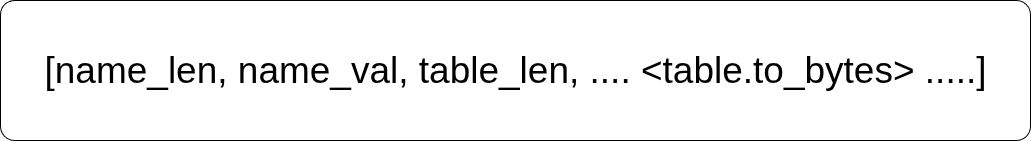
\includegraphics[width=0.6\textwidth]{gambar/bab4/urutan-penyimpanan-skema.png}
	\caption{Urutan penyimpanan Schema dalam \emph{byte}}
	\end{figure}


	\begin{enumerate}
		\item name\_len \\
		merupakan dari panjang atribut name yang disimpan dalam bentuk u8. \emph{Bytes} yang disimpan dibuat dengan panjang 8 mengikuti aturan primitif pada isize di bahasa pemrograman rust.
		
		\item name\_val \\
		merupakan value dari atribut name yang disimpan dalam bentuk u8. Panjang \emph{bytes} ini dapat berbeda-beda bergantung dengan isi dari nilainya. 

		\item table\_len \\
		merupakan dari panjang data tersimpan pada atribut tables yang disimpan dalam bentuk u8. Panjang penyimpanan juga mengikuti seperti apa yang telah di kutip di name\_len

		\item table.to\_bytes \\
		Urutan dilanjutkan memanggil \emph{method} to.bytes pada setiap data tersimpan pada atribut tables
	\end{enumerate}


	\item to\_data \\
	Method ini berguna untuk mengembalikan data yang telah disimpan pada \emph{method} to\_bytes dari bentuk vector u8 menjadi \emph{class} yang sebelumnya disimpan pada \emph{filesystem}. 
  Sehingga proses pengembaliannya merupakan kebalikan dari proses yang ada pada \emph{method} to\_bytes. \emph{Method} ini mengembalikan tipe data schema yang telah berisikan data. \emph{Method} ini bersifat
  static.

	\item save \\	
	Method ini digunakan untuk melakukan proses penyimpanan dari vector \emph{bytes} ke dalam \emph{filesystem}. Di dalam \emph{method} save, \emph{method} to\_bytes akan dipanggil dan return dari \emph{function} tersebut
  yang akan disimpan pada \emph{filesystem}. File disimpan ke dalam \emph{filesystem} dalam \emph{folder} schema, dan \emph{file} tersebut dinamakan dengan nama schema yang telah dibuat. \emph{Method} save ini nanti 
  juga akan selalu dipanggil setiap ada perubahan data seperti create, update dan juga delete untuk menunjang integritas data.

	\item add\_table \\
	Method yang berguna untuk menambah jumlah table yang disimpan pada \emph{class} Schema. Di dalam \emph{method} ini juga terdapat pengecekkan keunikan nama tabel. Jika terdapat tabel baru yang memiliki
  nama yang sama, maka \emph{method} ini akan mengembalikan error.

	\item add\_column\_to\_table \\
	Method yang berguna untuk menambahkan sebuah kolom baru pada tabel yang dituju.

	\item list\_column\_on\_table \\
	Method yang berguna untuk menampilkan kolom-kolom pada tabel yang dituju.
			

	\item search\_table \\
	Method yang berguna untuk mencari tabel yang terdapat dalam schema.

	\item check\_table\_index \\
	Method yang berguna untuk menampilkan \emph{index} atau urutan tabel di dalam vector table berdasarkan nama tabel pada \emph{parameter}.

	\item delete\_table \\
	Method yang berguna untuk menghapus tabel berdasarkan nama pada \emph{parameter}.
  
	\item add\_data \\
	Method yang berguna untuk menambah data baru berdasarkan tabel yang telah disimpan pada \emph{database}.
  
	\item get\_data \\
	Method yang berguna untuk menampilkan semua data yang telah tersimpan pada tabel yang dituju.

	\item search\_data \\
	Method yang berguna untuk menampilkan pencarian data berdasarkan kolom-kolom pada tabel yang dituju.

	\item update\_data \\
	Method yang berguna untuk mengubah data berdasarkan kondisi yang ada pada \emph{parameter}. Data yang diubah adalah data yang juga ditentukan 
  pada \emph{parameter}.

	\item delete\_data \\
	Method yang berguna untuk menghapus data berdasarkan kondisi yang ada pada \emph{parameter}.

	\item join\_table \\
	Berguna untuk melihat data antar tabel yang dihubungkan melalui kolom yang telah dibuat pada saat pembuatan tabel. \emph{Method} ini berguna sebagai
  pengondisian pemanggilan \emph{method} berdasarkan tipe \emph{join} yang tersedia pada \emph{database engine} ini yaitu \emph{inner} \emph{join}, \emph{left} \emph{join} dan \emph{right} \emph{join}.

	\item left\_right\_join\_table \\
	Method yang berguna untuk melakukan \emph{left} atau \emph{right} \emph{join}. Perbedaan proses dari \emph{left} dan \emph{right} \emph{join} terletak hanya pada \emph{parameter} dari \emph{method} ini.
  
	\item join\_inner\_table \\
	Method yang berguna untuk melakukan \emph{inner} \emph{join}.
  
	\item build\_index \\
	Method yang berguna untuk membangun \emph{index} berdasarkan data \emph{index} yang telah disimpan pada \emph{file} \emph{index}. \emph{Method} ini dipanggil di dalam \emph{method} to\_data.

	\item save\_index \\
	Method yang berguna untuk menyimpan \emph{index} ke dalam \emph{filesystem}. \emph{Index} ini disimpan ke \emph{file} didalam \emph{folder} \emph{index}. Nama dari \emph{file} tersebut juga akan
  disamakan dengan nama schema yang telah dibuat.

	\item clear\_index \\
	Method yang berguna untuk membersihkan  atau menghapus \emph{index} yang telah disimpan. \emph{Method} ini selalu dipanggil di dalam \emph{method} save.
  
	\item get\_file \\
	Sebuah \emph{method} yang bersifat private, berguna untuk mengembalikan Object File berdasarkan nama yang ada pada \emph{parameter}. 
  \emph{Method} ini di panggil di dalam \emph{method} build\_index.

	\item list\_all\_table \\
	Method yang berguna untuk menampilkan nama tabel yang tersimpan pada schema dalam bentuk vector string.

	\item print \\
	Method yang digunakan hanya pada saat pengembangan berlangsung, berguna untuk menampilkan data pada terminal tempat \emph{database engine} di jalankan.
\end{enumerate}

\subsection{Table}
Class Table merupakan \emph{class} yang merepresentasikan sebuah tabel dalam \emph{database}. Berikut adalah gambar \emph{class} diagram dari \emph{class} Table:
\begin{figure}[H]
  \centering{}
	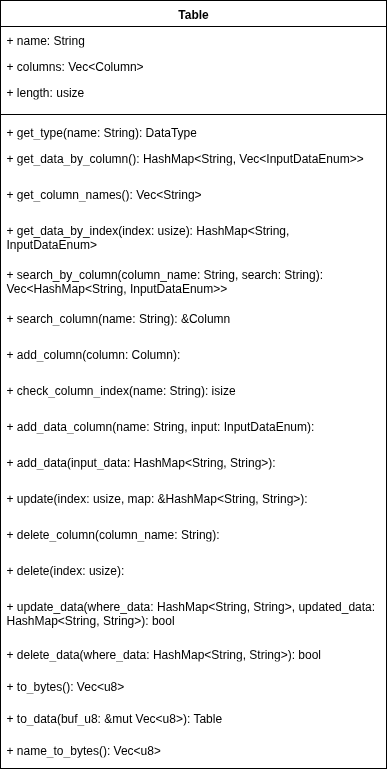
\includegraphics[width=0.6\textwidth]{gambar/bab4/Table}
  \caption{Class Diagram Table}
\end{figure}

Atribut dan \emph{method} yang tertulis pada \emph{class} diagram berguna untuk melakukan pengolahan data dari satu entitas Table. Sebagian besar dari atribut dan \emph{method} ini
dipanggil pada \emph{class} Schema. Terdapat 3 attribut pada \emph{class} Schema, yaitu:

\begin{enumerate}
	\item name \\
	Berguna untuk menyimpan nama dari tabel dalam bentuk tipe data string.

	\item columns \\
	Attribut ini berguna untuk menyimpan list kolom pada tabel yang dibuat. Tipe data atribut ini adalah Vector berisi \emph{class} Column, yang akan 
  dijelaskan pada pembahasan \emph{class} berikutnya. 

	\item length \\
	Berguna untuk menyimpan panjang dari vector columns. Atribut ini dapat dikatanak menyimpan panjang dari baris di tabel.
\end{enumerate}

Setelah atribut, terdapat method-method dalam \emph{class} Table yang berguna untuk mengolah data yang disimpan di dalam atribut. Terdapat 18 \emph{method} dalam \emph{class} Table, yaitu:

\begin{enumerate}
	\item get\_type \\
	Berguna untuk mengembalikan tipe data dari kolom yang dituju.

	\item get\_data\_by\_column \\
	Berguna untuk mengambalikan data-data yang tersimpan dalam kolom tabel dalam bentuk hashmap.

	\item get\_column\_names \\
	Berguna untuk melihat nama kolom yang tersimpan pada tabel dalam bentuk vector string.

	\item get\_data \\
	Berguna untuk mengambil seluruh data yang tersimpan pada satu \emph{class} Table.

	\item get\_data\_by\_index \\
	Method ini bersifat private, berguna untuk mengambil \emph{index} atau urutan data yang tersimpan pada tabel.

	\item search\_by\_column \\
	Method ini berguna untuk melakukan pencarian terhadap kolom yang dituju.

	\item search\_column \\
	Berguna untuk melakukan pencarian kolom berdasarkan nama kolom yang telah dibuat. 

	\item print \\
	Berfungsi sama seperti \emph{method} print yang ada pada \emph{class} Schema, berguna untuk menampilkan data yang tersimpan pada class
  Table di terminal tempat \emph{database engine} berjalan. \emph{Method} ini sering digunakan pada saat pengembangan saja.

	\item add\_column \\
	Berfungsi untuk menambah atau membuat kolom baru.

	\item check\_column\_index \\
	Berfungsi untuk mengembalikan \emph{index} atau urutan kolom yang tersimpan pada atribut columns.

	\item add\_data\_column \\
	Berfungsi untuk menambahkan 1 data pada suatu kolom, \emph{method} ini tidak digunakan dalam fitur \emph{database engine} ini karena dapat menghancurkan
  integritas antar kolom di sebuah tabel. Mungkin \emph{method} ini akan berguna di fitur yang akan datang.

	\item add\_data \\
	Berfungsi untuk menambahkan 1 baris data baru pada tabel.

	\item update \\
	Berfungsi untuk mengubah nilai atau isian pada 1 baris data yang dituju di sebuah tabel menggunakan \emph{index} atau urutan kolom pada tabel.

	\item delete\_column \\
	Berfungsi untuk menghapus kolom yang tersimpan pada tabel. Dengan menghapus kolom, maka semua data yang tersimpan pada kolom tersebut juga akan dihapus.
  Menggunakan nama kolom untuk mencari kolom yang dituju.

	\item delete \\
	Berfungsi untuk menghapus data pada tabel menggunakan \emph{index} atau urutan dari data yang telah tersimpan.
  
	\item update\_data \\
  Memiliki fungsi yang sama dengan \emph{method} update, namun menggunakan pencarian berdasarkan kolom-kolom yang ada pada tabel untuk mencari data yang ingin diubah.
  
	\item delete\_data \\
  Memiliki fungsi yang sama dengan \emph{method} delete, perbedaannya terletak pada pencariannya. \emph{Method} ini menggunakan kolom-kolom yang tersedia untuk menentukan
  baris data yang ingin dihapus.

	\item to\_bytes \\
  Memiliki fungsi yang sama dengan \emph{method} to\_bytes pada \emph{class} Schema, namun dikhususkan untuk mengubah \emph{class} Table saja. Proses pengubahan disimpan ke dalam vector
  u8 dengan urutan yang harus konsisten. Berikut adalah ilustrasi urutan penyimpanan dalam vector tersebut.

	\begin{figure}[H]
		\centering{}
			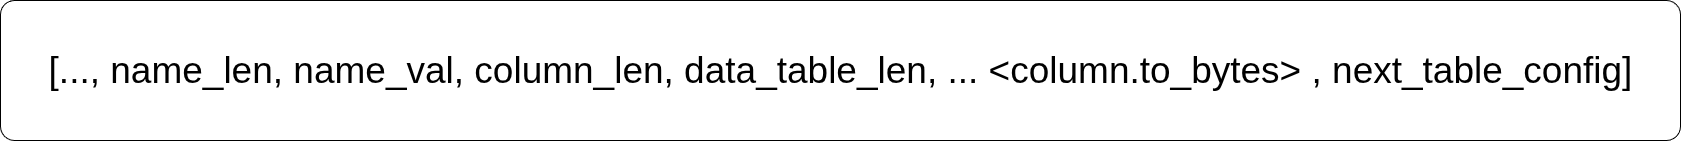
\includegraphics[width=0.6\textwidth]{gambar/bab4/urutan-penyimpanan-table.png}
		\caption{Urutan penyimpanan Table dalam byte}
		\end{figure}


	\begin{enumerate}
		\item name\_len \\
		merupakan dari panjang atribut name yang disimpan dalam bentuk u8. \emph{Bytes} yang disimpan dibuat dengan panjang 8 mengikuti aturan primitif pada isize di bahasa pemrograman rust.

		\item name\_val \\
		merupakan value dari atribut name yang disimpan dalam bentuk u8. Panjang \emph{bytes} ini dapat berbeda-beda bergantung dengan isi dari nilainya. 

		\item column\_len \\
		merupakan dari panjang data tersimpan pada atribut columns yang disimpan dalam bentuk u8. Panjang penyimpanan juga mengikuti seperti apa yang telah di kutip di name\_len

		\item data\_table\_len \\
		merupakan value dari atribut length yang disimpan dalam bentuk u8. Panjang \emph{bytes} ini juga mengikuti aturan pada name\_len. 

		\item column.to\_bytes \\
		Urutan dilanjutkan memanggil \emph{method} to.bytes pada setiap data tersimpan pada atribut columns

		\item \emph{next\_table\_config} \\
		Dilanjutkan dengan memanggil pengaturan tabel yang berikutnya.
	\end{enumerate}

	\item to\_data \\
  Proses yang berkebalikan dari \emph{method} to\_bytes, yaitu mengembalikan data dalam bentuk \emph{bytes} ke bentuk aslinya (class). Data yang dikembalikan dari \emph{method} ini 
  berupa \emph{class} Table.
  
	\item name\_to\_bytes \\
  \emph{Method} yang berfungsi untuk mengubah nama tabel ke dalam bentuk vector u8.
\end{enumerate}

\subsection{Column}
Class Column merupakan \emph{class} yang merepresentasikan sebuah kolom didalam sebuah tabel. Berikut adalah gambar \emph{class} diagram dari \emph{class} Column:
\begin{figure}[H]
  \centering{}
	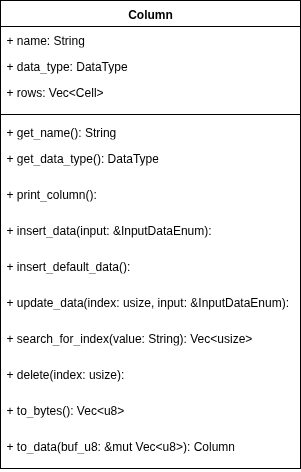
\includegraphics[width=0.6\textwidth]{gambar/bab4/Column}
  \caption{Class Diagram Column}
\end{figure}

Atribut dan \emph{method} yang tertulis pada \emph{class} diagram berguna untuk melakukan pengolahan data dari satu entitas Column. \emph{Class} Column dapat tersimpan dalam jumlah banyak di \emph{class} Table. 
Sebagian besar dari atribut dan \emph{method} ini juga akan dipanggil di \emph{class} Table. Terdapat 3 attribut pada \emph{class} Column, yaitu:

\begin{enumerate}
	\item name \\
	Berguna untuk menyimpan nama dari kolom dalam bentuk tipe data string.

	\item data\_type \\
	Attribut ini berguna untuk menyimpan tipe data dari sebuah kolom. Tipe data atribut ini adalah Enum DataType.

	\item rows \\
	Berguna untuk menyimpan data pada columns. Tipe data atribut rows meimiliki tipe vector yang berisi \emph{class} Cell.
\end{enumerate}

Selain atribut, \emph{class} Column ini juga memiliki \emph{method} yang berguna untuk mengolah data yang disimpan di atribut. Terdapat 10 \emph{method} di dalam \emph{class} Column, yaitu:

\begin{enumerate}
	\item get\_name \\
	Berguna untuk mengembalikan nama dari kolom.

	\item get\_data\_type \\
	Method yang berguna untuk mengembalikan tipe data dari data yang disimpan dalam \emph{class} Column.

	\item print\_column \\
	Method ini hanya dipakai pada saat pengembangan, dan memiliki fungsional yang sama seperti print \emph{method} di \emph{class} Schema dan \emph{class} Table. Berfungsi untuk menampilkan
  data yang disimpan pada terminal tempat \emph{database engine} dijalankan.

	\item insert\_data \\
	Method ini berguna untuk membuat data baru pada kolom. Data baru yang masuk ke dalam kolom harus disesuaikan dengan tipe data yang ada pada atribut data\_type.

	\item insert\_default\_data \\
	Method ini berguna untuk membuat data baru pada kolom dengan nilai default. String kosong untuk tipe data string dan nilai 0 untuk tipe data integer. Hal ini dibuat
  jika pengguna tidak mendefinisikan nilai pada kolom yang ada pada tabel saat menambahkan data baru.
  
	\item update\_data \\
	Berguna untuk mengubah data yang tersimpan pada atribut rows. \emph{Method} ini dipanggil di dalam \emph{method} update di \emph{class} Table.
  
	\item search\_for\_index \\
	Berguna untuk mengembalikan \emph{index} dari sebuah data yang tersimpan pada atribut rows. Rows yang dikembalikan adalah rows yang memiliki value yang ada di \emph{parameter}.
  \emph{Method} ini dapat mengembalikan indeks lebih dari 1 dalam bentuk vector.
  
	\item delete \\
	Berguna untuk menghapus data berdasarkan urutan atau indeks yang tersimpan pada atribut rows.
  
	\item to\_bytes \\
	Sama seperti \emph{method} di \emph{class} sebelumnya, berguna untuk mengubah data tersimpan ke dalam bentuk \emph{bytes} atau vector u8. Proses penyimpan ke dalam vector memiliki urutan
  yang harus sesuai. Berikut adalah ilustrasi urutan yang disimpan dalam vector.

  \begin{figure}[H]
	\centering{}
		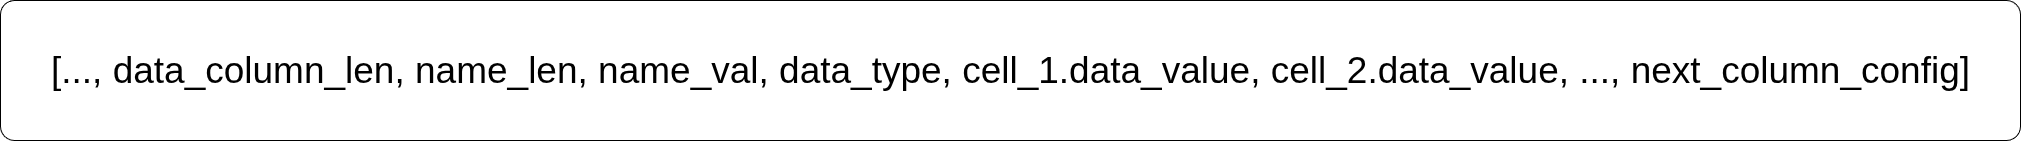
\includegraphics[width=0.8\textwidth]{gambar/bab4/urutan-penyimpanan-column.png}
	\caption{Urutan penyimpanan Column dalam byte}
	\end{figure}

	\begin{enumerate}
		\item data\_column\_len \\
		merupakan dari panjang data tersimpan pada atribut rows yang disimpan dalam bentuk u8. \emph{Bytes} yang disimpan dibuat dengan panjang 8 mengikuti aturan 
		primitif pada isize di bahasa pemrograman rust.

		\item name\_len \\
		merupakan dari panjang data dari atribut name yang disimpan dalam bentuk u8. Panjang penyimpanan juga mengikuti seperti apa yang telah di kutip di data\_column\_len

		\item name\_val \\
		merupakan value dari atribut name yang disimpan dalam bentuk u8. Panjang \emph{bytes} ini dapat berbeda-beda bergantung dengan isi dari nilainya. 

		\item data\_type \\
		Berguna untuk menyimpan tipe data dari kolom. Pada urutan ini jika bernilai 0 maka tipe data dari kolom nya adalah 0, dan jika bernilai 1 maka bernilai integer.


		\item cell.data\_value \\
		Urutan dilanjutkan dengan melakukan for loop dan memanggil atribut data\_value pada setiap cell yang disimpan di dalam atribut rows. Karena atribut data\_value sudah berupa vector u8 maka
		nilainya bisa langsung dimasukkan ke dalam vector. Namun terdapat sedikit perbedaan proses pada string, karena harus menambah panjang dari value string yang tersimpan terlebih dahulu
		sebelum menyimpan nilai aslinya. 

		\item \emph{next\_column\_config} \\
		Dilanjutkan dengan memanggil pengaturan kolom yang berikutnya.
	\end{enumerate}
  
	\item to\_data \\
	Berfungsi untuk mengembalikan data kolom yang telah diubah ke \emph{bytes} menjadi data \emph{class} Column kembali.
\end{enumerate}

\subsection{Cell}
Class Cell merupakan \emph{class} yang merepresentasikan sebuah nilai yang tersimpan pada satu baris tabel. \emph{Class} Cell dibutuhkan karena, setiap nilai yang tersimpan dalam database
dapat memiliki tipe data yang berbeda-beda. Sehingga diperlukan sebuah \emph{class} kembali untuk menentukan hal tersebut. Berikut adalah gambar \emph{class} diagram dari \emph{class} Cell:
\begin{figure}[H]
  \centering{}
	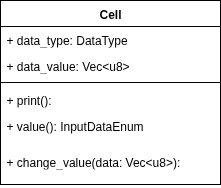
\includegraphics[width=0.6\textwidth]{gambar/bab4/Cell}
  \caption{Class Diagram Cell}
\end{figure}

Class Cell memiliki atribut dan beberapa \emph{method} yang berguna untuk menunjang fitur pada \emph{database engine}. Terdapat 2 attribut dalam \emph{class} Cell, yaitu:
\begin{enumerate}
	\item data\_type \\
	Berguna untuk menyimpan tipe data dari sebuah cell. Atribut ini memiliki tipe data Enum DataType dan berfungsi untuk memvalidasi tipe data yang ada pada cell
  dan \emph{class} Column tempat cell disimpan.  

	\item data\_value \\
	Berguna untuk menyimpan nilai atau value dari sebuah cell. Nilai atribut ini disimpan dalam bentuk vector u8. Tujuan dibuat seperti ini dikarenakan nilai yang disimpan
  dalam sebuah cell dapat memiliki tipe yang berbeda-beda.  Selain itu, dengan menggunakan vector u8 sebagai nilai dari atribut ini, proses penyimpanan ke \emph{filesystem} menjadi lebih
  karena dapat dilakukan tanpa perlu mengubahnya terlebih dahulu. 
\end{enumerate}

Atribut yang disimpan dalam sebuah Cell harus diolah agar dapat dikelola oleh \emph{database engine}. Dengan menggunakan method, kita dapat mengolah atribut agar dapat digunakan pada
fitur \emph{database engine}. Terdapat 3 \emph{method} yang terdapat pada \emph{class} Cell, yaitu:

\begin{enumerate}
	\item print \\
	Method yang berguna selama pengembangan \emph{database engine}. Berguna untuk menampilkan value dalam cell di terminal tempat \emph{database engine} dijalankan.  

	\item value \\
  Berguna untuk mengembalikan value dari bentuk \emph{byte} ke Enum InputDataEnum. Hal ini diperlukan karena nilai yang tersimpan dalam cell adalah \emph{bytes}, sehingga membutuhkan pemrosesan
  kembali ke tipe data asli nya. 

	\item change\_value \\
  Berguna untuk mengubah value yang tersimpan pada atribute data\_value sesuai dengan yang ada pada \emph{parameter}. Data dalam \emph{parameter} juga sudah dalam bentuk vector u8. 
\end{enumerate}

\subsection{Enumeration}
Terdapat beberapa nilai enum yang digunakan sebagai penyimpanan tipe data dalam \emph{database}. Terdapat 2 Enum class, yaitu:
\begin{enumerate}
	\item InputDataEnum \\
  Enum ini berguna untuk menyimpan data dalam bentuk String, Integer dan juga Null. Namun pada fitur \emph{database} kali ini, hanya 2 tipe data saja yang baru didukung untuk penyimpanannya
  yaitu String dan Integer. Khusus untuk enum ini, akan menggunakan library bernama serde dan serde\_derive untuk melakukan \emph{Serialization} dan \emph{Deserialization}. Hal ini diperlukan saat sedang
  melakukan penyimpanan \emph{index}, karena \emph{index} disimpan dalam bentuk HashMap. Dengan menggunakan library ini Hashmap yang berisi InputDataEnum dapat berubah ke dalam bentuk \emph{bytes} secara langsung
  tanpa perlu mengubahnya secara manual. Selain library serde dan serde\_derive, terdapat 1 macro lagi yang diterapkan pada enum ini yaitu Debug. Macro ini berguna agar value yang memiliki tipe InputDataEnum dapat
  dilihat hasilnya di terminal.
	
	\item DataType \\
  Enum yang berguna untuk menentukan tipe kolom yang tersimpan pada tabel dan tipe Cell yang tersimpan pada kolom.
\end{enumerate}

\subsection{Utils}
Selain beberapa \emph{class} inti, terdapat beberapa \emph{function} tambahan yang berguna untuk menunjang fitur-fitur yang tersedia pada \emph{database engine}. Semua \emph{function} ini tersimpan secara statis
pada \emph{file} utils.rs. Namun tidak semua \emph{function} dalam utils digunakan dalam penerapa fitur \emph{database engine}, sebagian hanya digunakan saat hendak melakukan debugging atau saat hendak melakukan
percobaan.

\subsection{DatabaseInterface}
Class \emph{DatabaseInterface} ini berfungsi sebagai penentu \emph{method} atau \emph{function} mana saja didalam \emph{database} yang dapat dijalankan oleh pengguna. Oleh karena itu, method-method di dalam class
ini hanya meneruskan paramater yang diterima ke \emph{method} yang ada dalam \emph{class} Schema sesuai dengan nama dari methodnya. Berikut adalah \emph{class} Diagram \emph{DatabaseInterface}.

\begin{figure}[H]
  \centering{}
	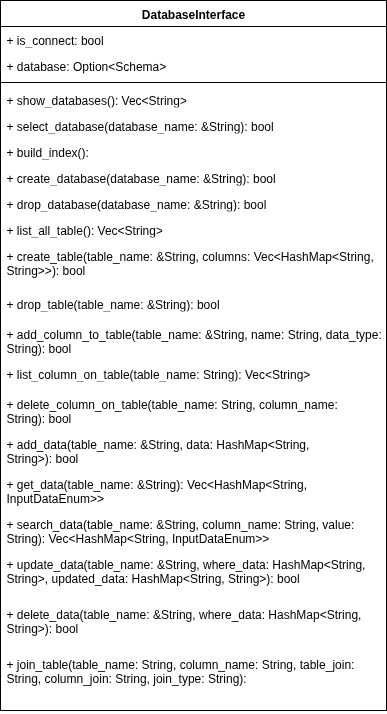
\includegraphics[width=0.6\textwidth]{gambar/bab4/DatabaseInterface.png}
  \caption{Class Diagram \emph{DatabaseInterface}}
\end{figure}

Perlu diperhatikan bahwa sebagian method-method di dalam \emph{class} ini, terutama
yang berhubungan dengan pengolahan data dalam database, memiliki validasi atau pengecekan apakah \emph{class} \emph{DatabaseInterface} sudah terhubung dengan \emph{class} Schema. \emph{Class} \emph{DatabaseInterface} ini memiliki
2 atribut yaitu:
\begin{enumerate}
	\item is\_connect \\
  Atribut dengan tipe data boolean untuk menentukan apakah instance schema sudah terhubung atau belum.
	
	\item database \\
  Atribut dengan tipe Option yang akan berisi instance dari \emph{class} Schema dan dapat berisi None jika instance Schema belum terhubung.
\end{enumerate}

Selain sebagai penentu method, terdapat mehod lain yang terdapat pada \emph{DatabaseInterface}. Berikut adalah method-method tambahan yang ada pada \emph{DatabaseInterface}:
\begin{enumerate}
	\item show\_databases \\
  \emph{Method} ini berguna untuk melihat list \emph{database} yang tersimpan dalam bentuk \emph{file} di \emph{folder} schema.

	\item select\_database \\
  \emph{Method} ini berguna untuk memilih \emph{database} dan memasukkannya ke dalam atribute \emph{database}.

	\item create\_database \\
  Berguna untuk membuat \emph{database} dan memanggil \emph{function} save di dalam \emph{class} Schema sehingga sebuah \emph{file} baru dibuat di dalam \emph{folder} schema sesuai dengan
  nama \emph{database} yang dimasukkan dalam \emph{parameter}.

	\item drop\_database \\
  Berguna untuk menghapus \emph{database} dengan cara menghapus \emph{file} \emph{database} pada \emph{folder} schema dan \emph{folder} \emph{index}.

	\item join\_data \\
	Terdapat sedikit perbedaan pada proses yang terjadi di dalam \emph{method} join\_data ini. Isi \emph{method} ini akan dijelaskan 
	lebih secara khusus pada sub bab 4.1.10 tentang \emph{indexing}
	
\end{enumerate}

\subsection{\emph{Indexing} pada fitur Join}
Penerapan fitur \emph{indexing} pada \emph{database engine} ini dilakukan pada fitur \emph{join}. Prinsip penerapannya sama seperti \emph{cache} pada umumnya. Hashmap digunakan
untuk mengumpulkan \emph{index} dengan menggunakan key dari \emph{parameter} yang dijalankan saat hendak menjalankan \emph{join}. Jika key dari \emph{parameter} tersedia dalam Hashmap, maka value dari
key tersebut akan dikembalikan. Sementara jika key tersebut tidak tersedia, maka akan memanggil \emph{method} join\_data yang ada pada \emph{class} Schema. Alur lebih detail terkait 
penerapan \emph{indexing} dapat dilihat pada \emph{method} join\_data pada \emph{class} \emph{DatabaseInterface}. Namun untuk penerapan \emph{indexing} saat ini masih belum berjalan dengan baik,
dikarenakan value disimpan dalam HashMap, dimana HashMap tersebut merupakan library bawaan dari rust. Value yang dikembalikan dari HashMap tersebut merupakan sebuah reference
dari value yang disimpan. Sementara nilai yang berupa reference tidak bisa di kembalikan atau di return dalam \emph{function} di bahasa pemrograman Rust. Untuk melakukan hal tersebut,
membutuhkan sebuah fitur yang bernama lifetime dan fitur lifetime ini masih belum bisa dikuasai penulis saat ini. Maka dari itu fitur join\_table bisa berjalan dan mengembalikan data
jika fitur \emph{indexing} ini dimatikan. Jika hanya ingin melihat isi data dari hasil \emph{indexing}, dapat menggunakan \emph{method} println! pada rust. Untuk penyimpanan \emph{HashMap} dalam \emph{filesystem}, 
akan menggunakan library bernama \emph{bincode}. Karena proses pengubahan dari data ke byte yang saat ini dibuat, hanya ditujukan
bagi \emph{class} schema, table dan column. 


\subsection{DatabaseConnection}
Class \emph{DatabaseConnection} merupakan \emph{class} yang berguna untuk \emph{database engine} melakukan koneksi ke sistem lain. \emph{Class} ini menggunakan 
DatabaseInterface sebagai penghubung ke \emph{class} Schema untuk menjalankan fungsi-fungsi \emph{database}. Seperti yang dikutip pada sub bab 3.7 bahwa untuk
melakukan koneksi eksternal dengan sistem lain, \emph{database engine} akan menggunakan D-Bus. Pada penelitian ini, penerapan D-Bus di \emph{database} akan menggunakan
library atau biasa disebut crates dalam bahasa rust. Crates tersebut bernama zbus. Untuk menggunakan zbus pada \emph{class} \emph{DatabaseConnection}, penerapan macro
interface diperlukan. Hal ini sesuai dengan petunjuk yang ada pada dokumentasi zbus. Lalu \emph{library} bernama tokio akan digunakan
untuk membuat \emph{connection} menggunakan zbus pada function main di \emph{file} main.rs. Berikut adalah \emph{class} diagram dari \emph{class} \emph{DatabaseConnection}.


\begin{figure}[H]
  \centering{}
	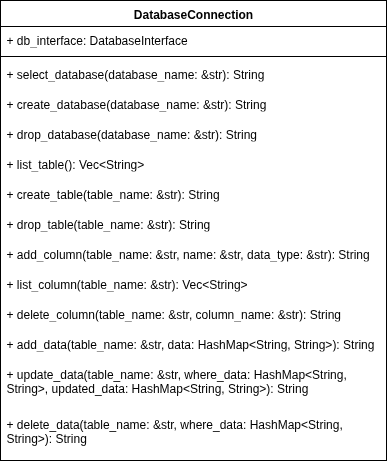
\includegraphics[width=0.6\textwidth]{gambar/bab4/DatabaseConnection}
  \caption{Class Diagram Column}
\end{figure}

Class \emph{DatabaseConnection} memiliki sebuah atribut bernama db\_interface. Atribut ini memiliki tipe data dari class
DatabaseInterface, yang berguna untuk memastikan bahwa \emph{class} \emph{DatabaseConnection} sudah terhubung dengan \emph{class} Schema.
Karena pada saat pertama kali \emph{database engine} ini dinyalakan, \emph{database} atau schema harus dipilih terlebih dahulu untuk
menentukan di schema mana data akan diolah. Untuk memilih schema, dapat menggunakan \emph{method} select\_database yang terdapat
pada \emph{class} \emph{DatabaseInterface}.

Perlu diketahui bahwa koneksi dengan menggunakan D-Bus untuk \emph{database engine} saat belum mendukung semua fungsi-fungsi pada \emph{database}. Karena secara default, 
koneksi dengan D-Bus hanya mendukung beberapa tipe data yang ada pada Rust saja. Untuk tipe data \emph{class} yang dibuat sendiri, diperlukan pengaturan tambahan agar bisa
melakukan koneksi ke sistem lain. Diantara \emph{method} yang mengembalikan tipe \emph{class} pada \emph{class} \emph{DatabaseInterface} adalah get\_data, search\_data, dan join\_table.
Oleh karena itu implementasi ketiga \emph{method} tersebut masih belum didukung pada koneksi melalui D-Bus saat ini.

\section{Pengujian}

Untuk pengujian akan dilakukan dengan 2 skema, yaitu pengujian secara  menggunakan bahasa pemrograman yang sama 
(dalam penelitian ini menggunakan bahasa rust) dan pengujian secara eksternal dengan menggunakan D-Bus yang akan digunakan pengguna
untuk menjalankan fungsi \emph{database}. Pengujian terpisah ini dilakukan berdasarkan alasan yang terdapat pada sub bab 4.1.11, yaitu tidak semua \emph{method} di 
DatabaseInterface dapat diakses oleh pengguna melalui D-Bus. 

Untuk memudahkan dalam pelaksanaan ujian, pada \emph{file} main.rs sebuah \emph{function} baru akan dibuat untuk
masing pengujian internal dan pengujian internal dengan data hasil \emph{crawling}. \emph{Function} untuk pengujian internal bernama test dan \emph{function} untuk pengujian internal
dengan data dummy bernama test\_data\_crawling. Masing-masing \emph{function} tersebut akan menerapkan \emph{macro} bernama \emph{test}. \emph{Macro} ini merupakan \emph{macro}
bawaan dari \emph{rust}. Lalu untuk \emph{function} main dalam main.rs, akan berisi konfigurasi untuk menjalankan \emph{library} zbus untuk menerima koneksi dari luar.

\subsection{Pengujian Internal}
Pengujian internal dilakukan dengan membuat sebuah \emph{class} baru bernama TestDatabaseInterface. Karena pengujian dilakukan  maka \emph{method} print 
pada setiap \emph{class} yang telah dijelaskan di sub bab sebelumnya, akan digunakan. Pengujian akan dilakukan dengan menggunakan data \emph{Dummy} yang terdiri dari 
2 tabel yang saling berkaitan. Berikut adalah isi tabel dari data \emph{Dummy} yang digunakan. 

\begin{table}[H]
  \centering{}
  \begin{tabular}{|m{2.5cm}|m{4cm}|m{4cm}|}
      \hline
      \textbf{id (Integer)} & \textbf{first\_name (String)} &  \textbf{last\_name (String)} \\
      \hline
      0 & Farhan & Abdul \\
      \hline
      1 & Akbar & Maulana \\
      \hline
      2 & Daffa & Haryadi \\
      \hline
      3 & Hanif & Ramadhan \\
      \hline
      4 & Rudiansyah & Wijaya \\
      \hline
  \end{tabular}
  \caption{Tabel Users}
\end{table}


\begin{table}[H]
  \centering{}
  \begin{tabular}{|m{2cm}|m{2cm}|m{3cm}|m{3cm}|}
      \hline
      \textbf{id (Integer)} & \textbf{user\_id (Integer)} & \textbf{title (String)} &  \textbf{description (String)} \\
      \hline
      0 & 0 & Judul 0 & \emph{Long Text} \\ 
      \hline
      1 & 0 & Judul 1 & \emph{Long Text} \\ 
      \hline
      2 & 1 & Judul 2 & \emph{Long Text} \\ 
      \hline
      3 & 2 & Judul 3 & \emph{Long Text} \\ 
      \hline
      4 & 2 & Judul 4 & \emph{Long Text} \\ 
      \hline
      5 & 2 & Judul 5 & \emph{Long Text} \\ 
      \hline
      6 & 3 & Judul 6 & \emph{Long Text} \\ 
      \hline
      7 & 2 & Judul 7 & \emph{Long Text} \\ 
      \hline
      8 & 2 & Judul 8 & \emph{Long Text} \\ 
      \hline
      9 & 2 & Judul 9 & \emph{Long Text} \\ 
      \hline
      10 & 1 & Judul 10 & \emph{Long Text} \\ 
      \hline
      11 & 1 & Judul 11 & \emph{Long Text} \\ 
      \hline
      12 & 2 & Judul 12 & \emph{Long Text} \\ 
      \hline
  \end{tabular}
  \caption{Tabel Posts}
\end{table}

Pada tabel posts, data yang digunakan pada kolom description akan diambil Faker API (\cite{faker}) supaya dapat berisi text yang panjang.
Lalu untuk kolom user\_id pada tabel posts, berguna untuk menghubungkan antara tabel posts dengan tabel users.
Pengujian dilakukan pada masing-masing \emph{method} yang ada pada \emph{class} \emph{DatabaseInterface}. Berikut adalah \emph{class} diagram
dari \emph{class} \emph{TestDatabaseInterface}.

\begin{figure}[H]
  \centering{}
	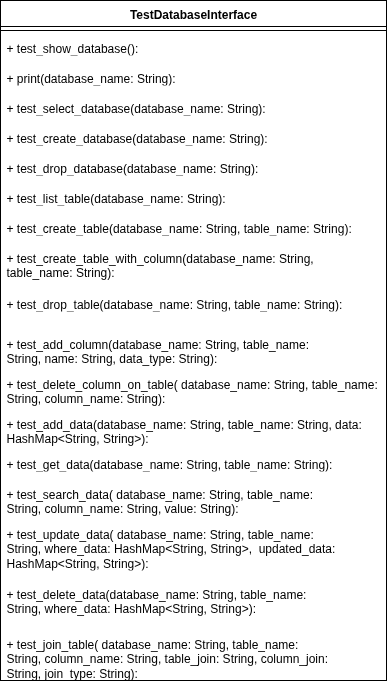
\includegraphics[width=0.6\textwidth]{gambar/bab4/TestDatabaseInterface.png}
  \caption{Class Diagram \emph{TestDatabaseInterface}}
\end{figure}

Pada penulisan ini pengujian akan berfokus pada fungsinal dasar \emph{database} yaitu membuat, melihat, mengubah dan menghapus data (CRUD).
Perlu diketahui bahwa pengujian yang dilakukan pada masing-masing \emph{function} dibuat dengan isian data yang sama satu sama lain. Lalu
terdapat sebuah informasi "Database berhasil terhubung" saat proses pengujian dibawah, dikarenakan proses \emph{database} harus terhubung terlebih dahulu
jika ingin menjalankan fungsinya. Jika terdapat tambahan seperti boolean true, juga penanda bahwa proses berhasil dijalankan.
Berikut ini adalah hasil pengujian database:

\begin{enumerate}
	\item test\_create\_database \\
  Pengujian dimulai dari mencoba melakukan pembuatan \emph{database}. \emph{Database} akan dibuat dengan nama articles. Dengan menjalankan \emph{function} ini
  maka akan terlihat sebuah \emph{file} baru dalam \emph{folder} schema dan \emph{folder} \emph{index}. File tersebut memiliki nama yang sama dengan \emph{database} yang dibuat.
  Pada terminal juga terdapat sebuah informasi bahwa \emph{database} berhasil terbuat.
  \begin{figure}[H]
  	\centering{}
	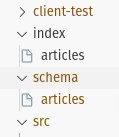
\includegraphics[width=0.3\textwidth]{gambar/bab4/test-create-database}
  	\caption{File baru telah terbuat dalam \emph{folder} \emph{index} dan schema}
  \end{figure}
	
	\item test\_select\_database \\
  \emph{Method} yang berguna untuk memilih \emph{database} terlebih dahulu. Karena tanpa melakukan pemilihan database, maka \emph{database engine} tidak akan berjalan.
  \emph{Database} yang dipilih adalah \emph{database} yang telah dibuat sebelumnya yaitu article. Jika pengujian ini berhasil maka akan muncul informasi bahwa
  \emph{database} berhasil terhubung.
   \begin{figure}[H]
  	\centering{}
	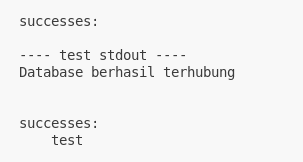
\includegraphics[width=0.6\textwidth]{gambar/bab4/test-select-database}
  	\caption{Informasi \emph{database} telah terhubung}
   \end{figure}

	\item test\_create\_table \\
  \emph{Method} yang berguna untuk membuat tabel pada \emph{database} yang dituju. Untuk kasus pengujian ini, vector kosong akan digunakan sebagai input dari kolom nya.
  Sehingga tabel yang terbuat adalah sebuah tabel tanpa kolom. \emph{Method} ini akan dijalankan 2x untuk menyesuaikan dengan data \emph{Dummy} yang terdapat pada tabel 4.1
  dan tabel 4.2. Nilai true pada gambar mengindikasikan bahwa pembuatan tabel telah berhasil.
  \begin{figure}[H]
  	\centering{}
	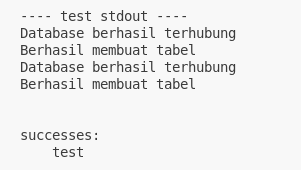
\includegraphics[width=0.6\textwidth]{gambar/bab4/test-create-table}
  	\caption{Informasi tabel telah berhasil terbuat}
   \end{figure}

	\item test\_add\_column \\
  Pengujian yang dilakukan untuk menambah kolom baru pada tabel yang telah dibuat. Kolom-kolom akan ditambahkan sesuai dengan nama dan tipe data yang ada pada tabel 4.1 dan tabel 4.2. 
  Oleh karena itu pengujian akan dilakukan sebanyak 7 kali menyesuaikan dengan jumlah kolom pada tabel yang disebutkan sebelumnya.
  \begin{figure}[H]
  	\centering{}
	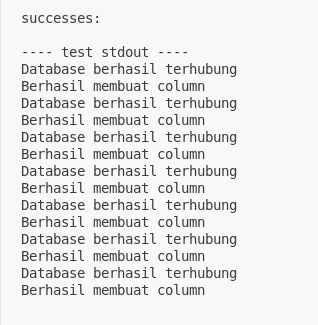
\includegraphics[width=0.3\textwidth]{gambar/bab4/test-create-column}
  	\caption{Informasi kolom telah berhasil terbuat}
   \end{figure}

	\item test\_add\_data \\
  Setelah berhasil membuat kolom, maka pengujian pembuatan dapat dilakukan. \emph{Method} pengujian ini akan membuat sebuah baris data baru di tabel dan kolom yang sudah dibuat. Jumlah dan 
  isian yang dibuat akan sama seperti data pada tabel 4.1 dan tabel 4.2.
  \begin{figure}[H]
  	\centering{}
	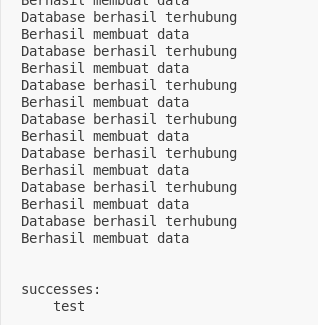
\includegraphics[width=0.4\textwidth]{gambar/bab4/test-create-data}
  	\caption{Informasi data telah berhasil terbuat}
   \end{figure}

	\item test\_get\_data \\
  Setelah berhasil membuat data, data yang telah disimpan akan diuji untuk proses pengambilannya. \emph{Method} ini akan menampilkan semua data pada tabel yang dituju dengan
  menggunakan \emph{method} print di dalam \emph{class} Table.
  \begin{figure}[H]
  	\centering{}
	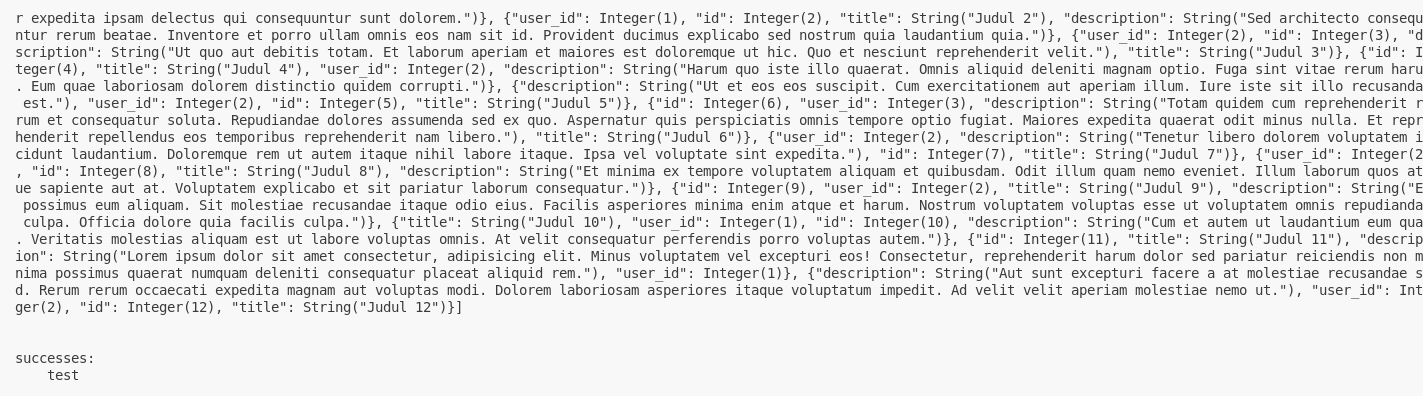
\includegraphics[width=0.6\textwidth]{gambar/bab4/test-get-data-posts.png}
  	\caption{Hasil data tabel \emph{posts} telah berhasil terbuat}
   \end{figure}
  \begin{figure}[H]
  	\centering{}
	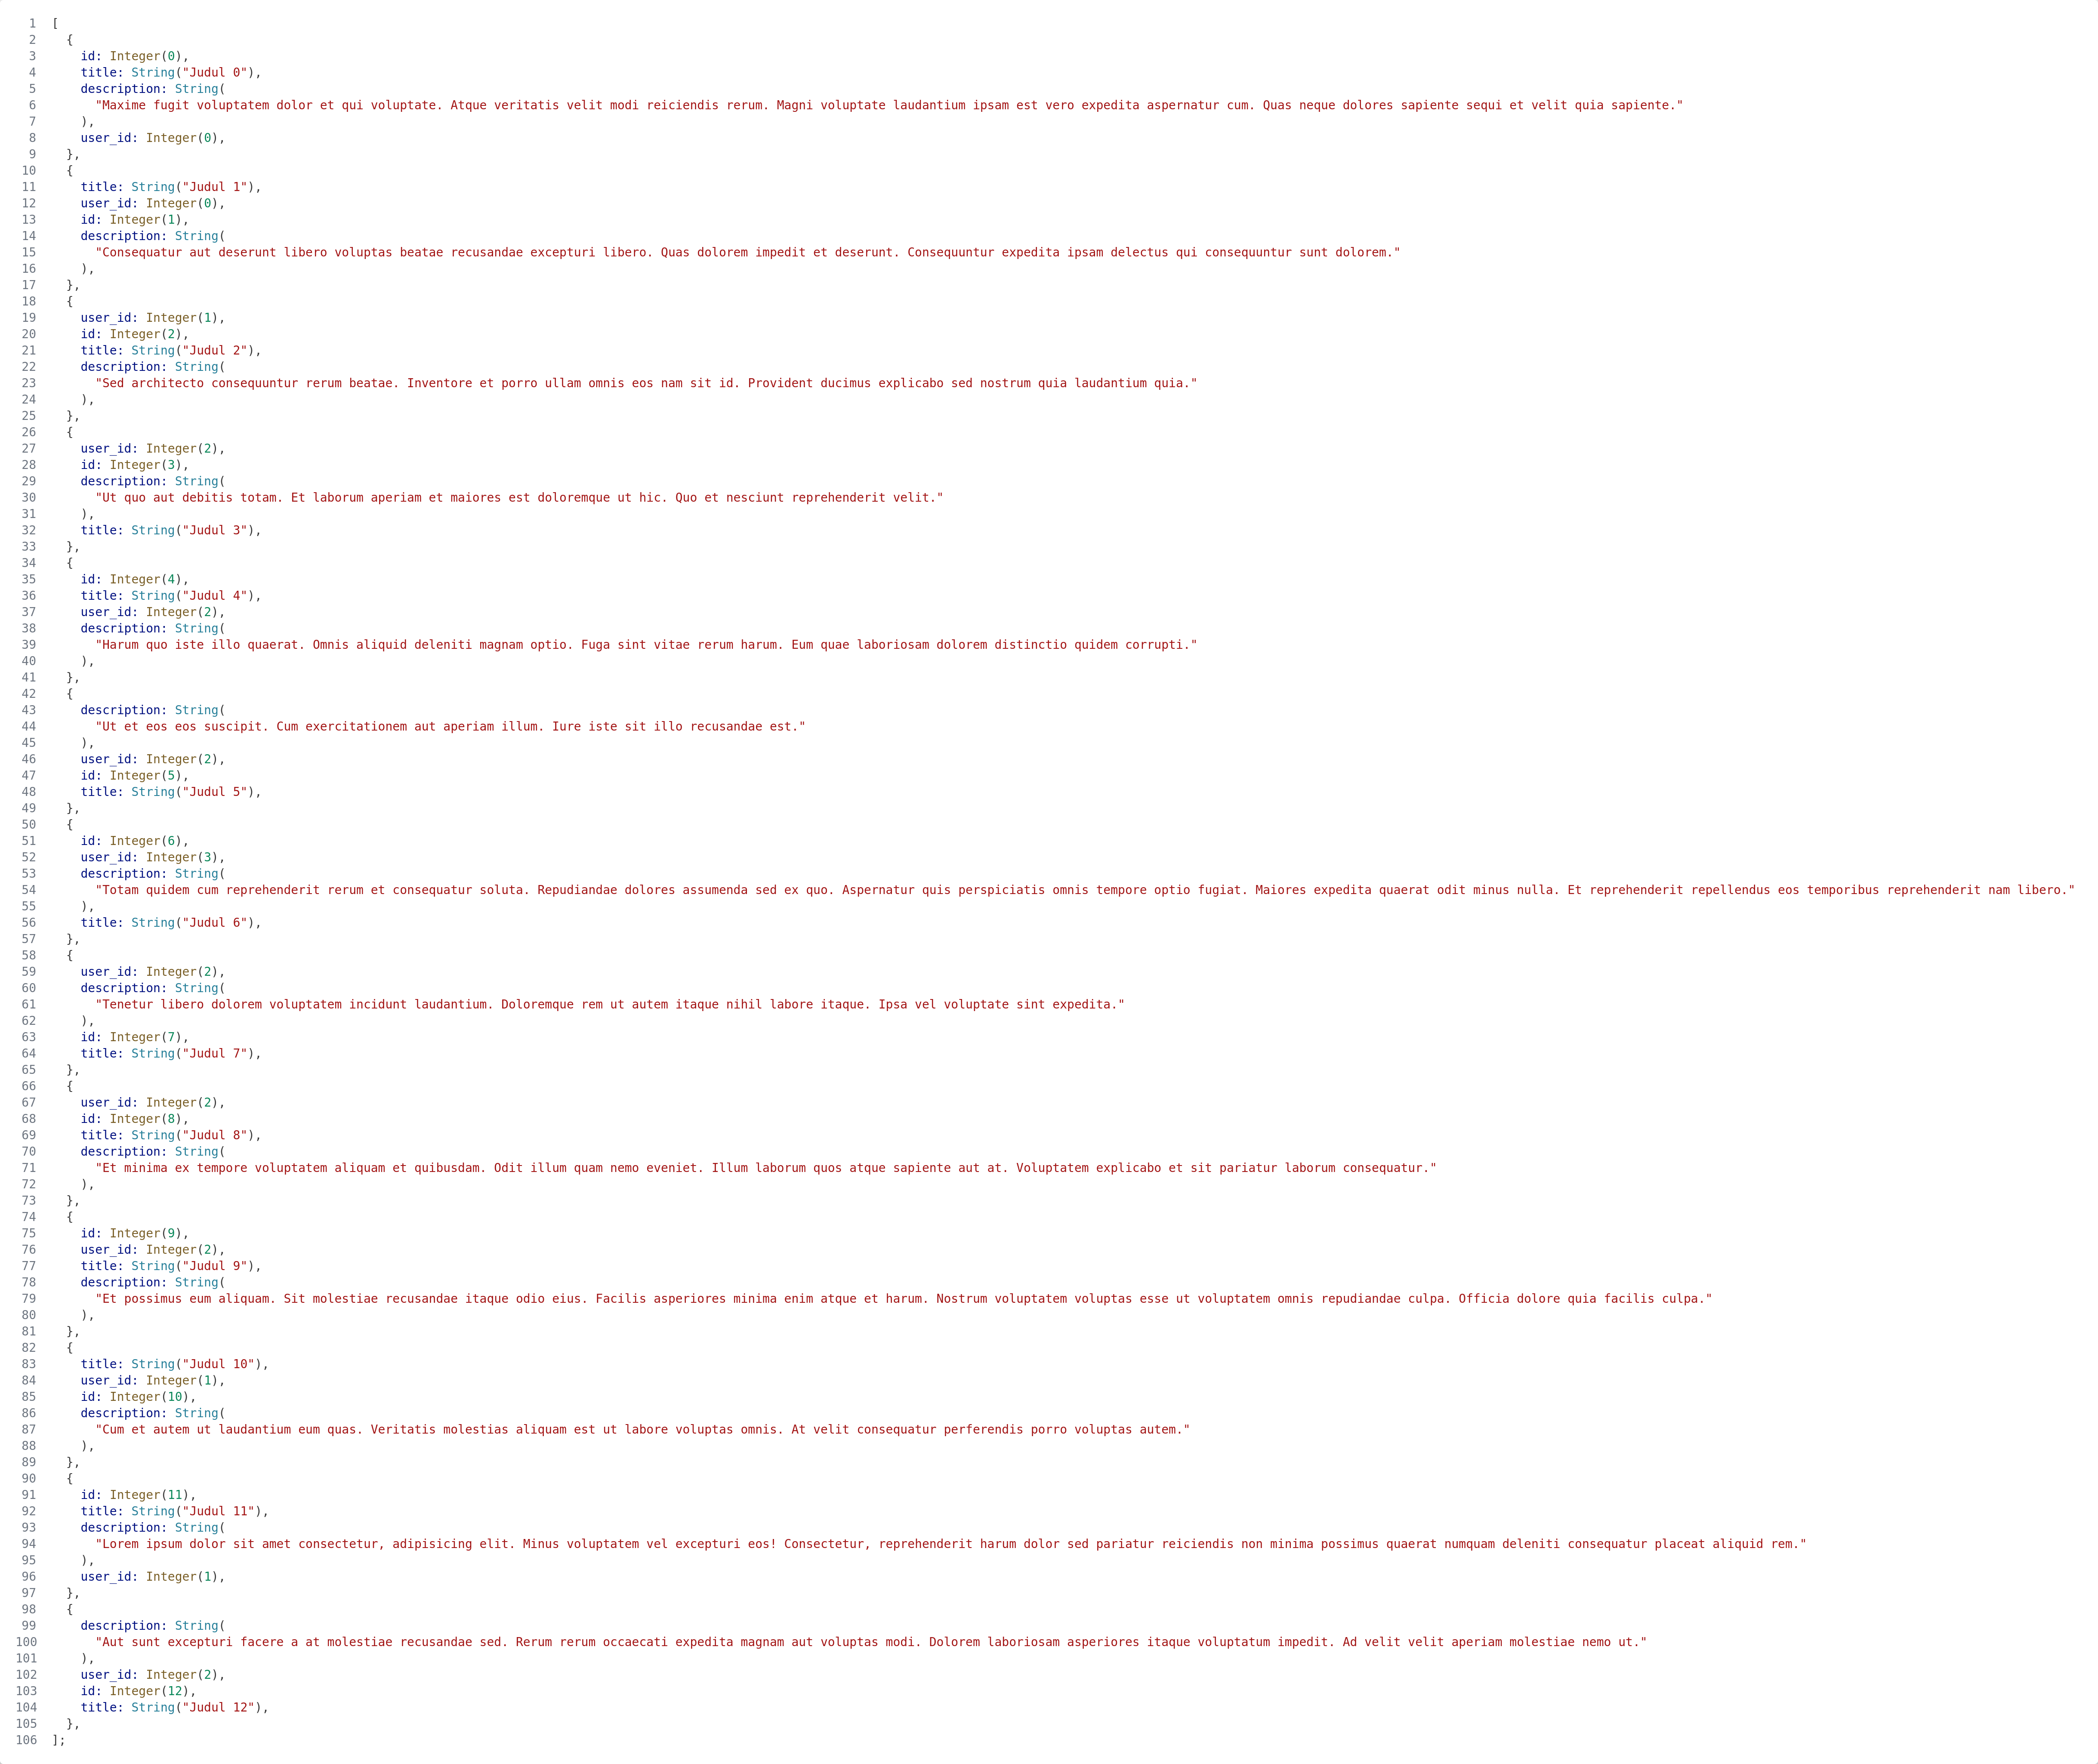
\includegraphics[width=0.9\textwidth]{gambar/bab4/test-get-data-posts-beautify.png}
  	\caption{Hasil data tabel \emph{posts} yang telah diformat menggunakan \emph{prettier} (\emph{Extension} \emph{Visual Studio Code} pada Javascript)}
   \end{figure}

  \begin{figure}[H]
  	\centering{}
	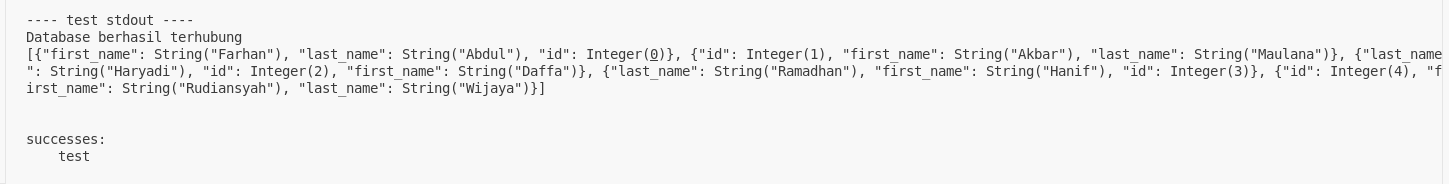
\includegraphics[width=0.6\textwidth]{gambar/bab4/test-get-data-users.png}
  	\caption{Hasil data tabel \emph{users} telah berhasil terbuat}
   \end{figure}
  \begin{figure}[H]
  	\centering{}
	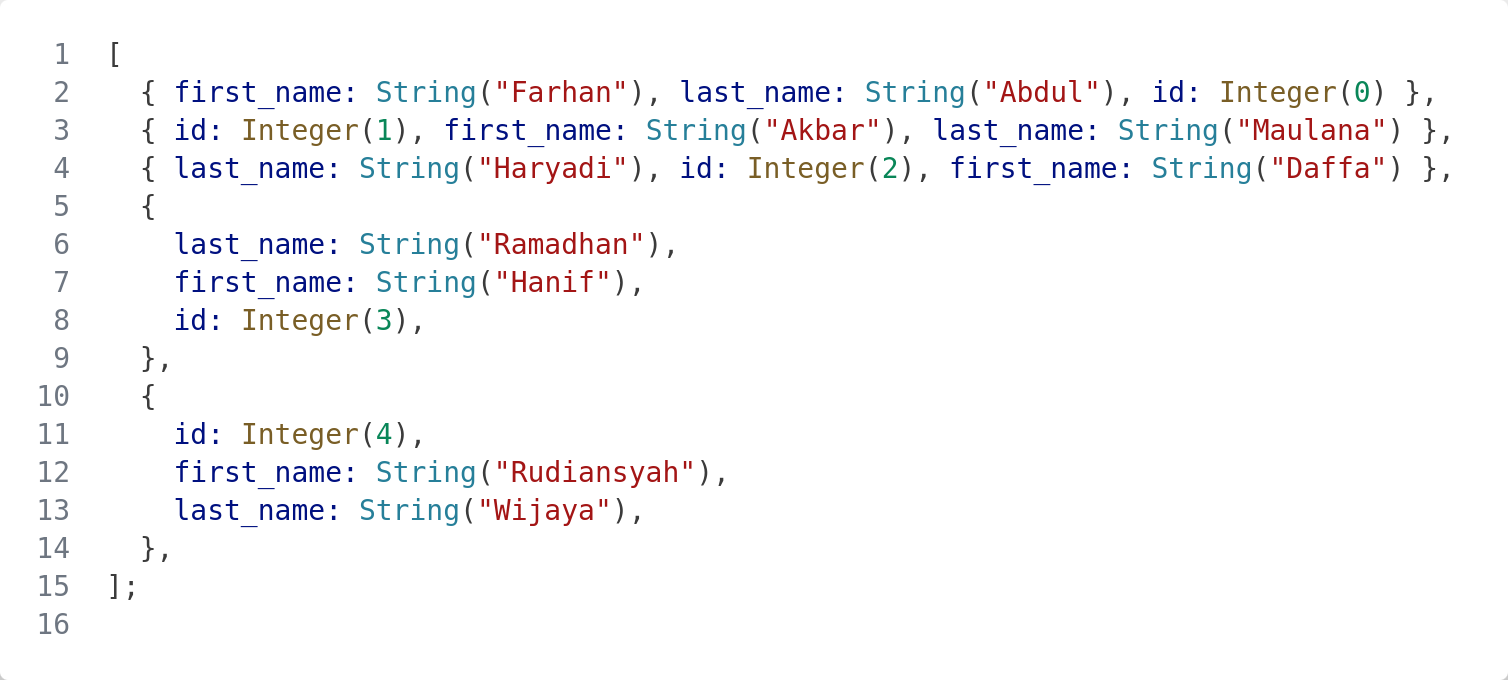
\includegraphics[width=0.9\textwidth]{gambar/bab4/test-get-data-users-beautify.png}
  	\caption{Hasil data tabel \emph{users} yang telah diformat menggunakan \emph{prettier} (\emph{Extension} \emph{Visual Studio Code} pada Javascript)}
   \end{figure}

	\item test\_update\_data \\
  \emph{Method} pengujian ini akan melakukan pengubahan pada data yang telah disimpan di \emph{database}. Pengujian ini membutuhkan \emph{parameter} untuk menentukan data mana yang akan dihapus, dan data apa saja
  yang akan diubah. Untuk kasus uji kali ini, akan mengubah kolom pada tabel users yang memiliki id dengan value 0 dan first\_name yang memiliki value "Farhan". Sementara data yang diubah adalah
  kolom last\_name, yang akan diubah berisi "Abdul Hamid".

  \begin{figure}[H]
  	\centering{}
	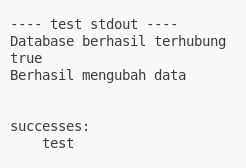
\includegraphics[width=0.6\textwidth]{gambar/bab4/test-update-data.png}
  	\caption{Informasi data berhasil diubah}
   \end{figure}

	\item test\_search\_data \\
  Pengujian \emph{method} search data ini dilakukan dengan memasukkan kolom dan value yang dituju. Data yang dicari adalah data pada tabel users yang memiliki id 0.
  \begin{figure}[H]
  	\centering{}
	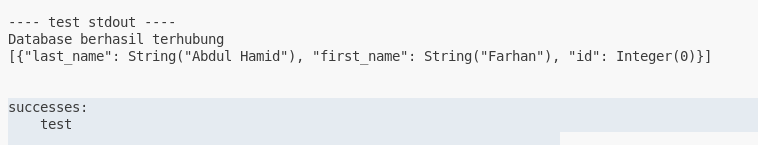
\includegraphics[width=0.6\textwidth]{gambar/bab4/test-search-data-users.png}
  	\caption{Informasi hasil pencarian}
   \end{figure}
    \begin{figure}[H]
  	\centering{}
	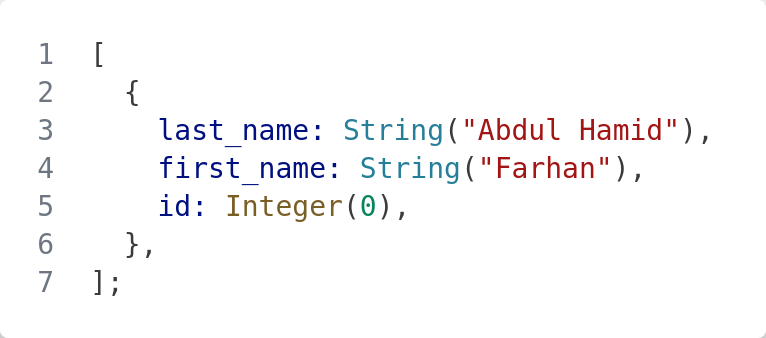
\includegraphics[width=0.7\textwidth]{gambar/bab4/test-search-data-users-beautify.png}
  	\caption{Hasil data yang telah diformat menggunakan \emph{prettier} (\emph{Extension} VSCode pada Javascript)}
   \end{figure}
  
  \item test\_join\_data \\
  Untuk menjalankan pengujian ini, kolom user\_id pada tabel posts akan digunakan untuk menyocokan data ke tabel users. Tabel, kolom serta tipe \emph{join} harus
  didefinisikan untuk menjalankan pengujian \emph{join} ini. Pada saat melakukan pengujian ini, terdapat beberapa error yang dialami dikarenakan \emph{index} yang tidak valid
  serta kesalahan dalam pengondisian \emph{join} nya. Namun untuk gambar dibawah, merupakan hasil dari implementasi yang telah diperbaiki.
  \begin{figure}[H]
  	\centering{}
	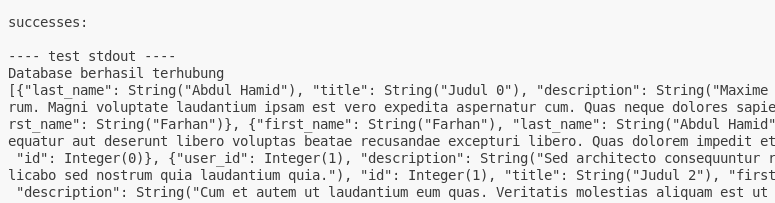
\includegraphics[width=0.6\textwidth]{gambar/bab4/test-join-data-inner.png}
  	\caption{Informasi hasil \emph{inner join}}
   \end{figure}
    \begin{figure}[H]
  	\centering{}
	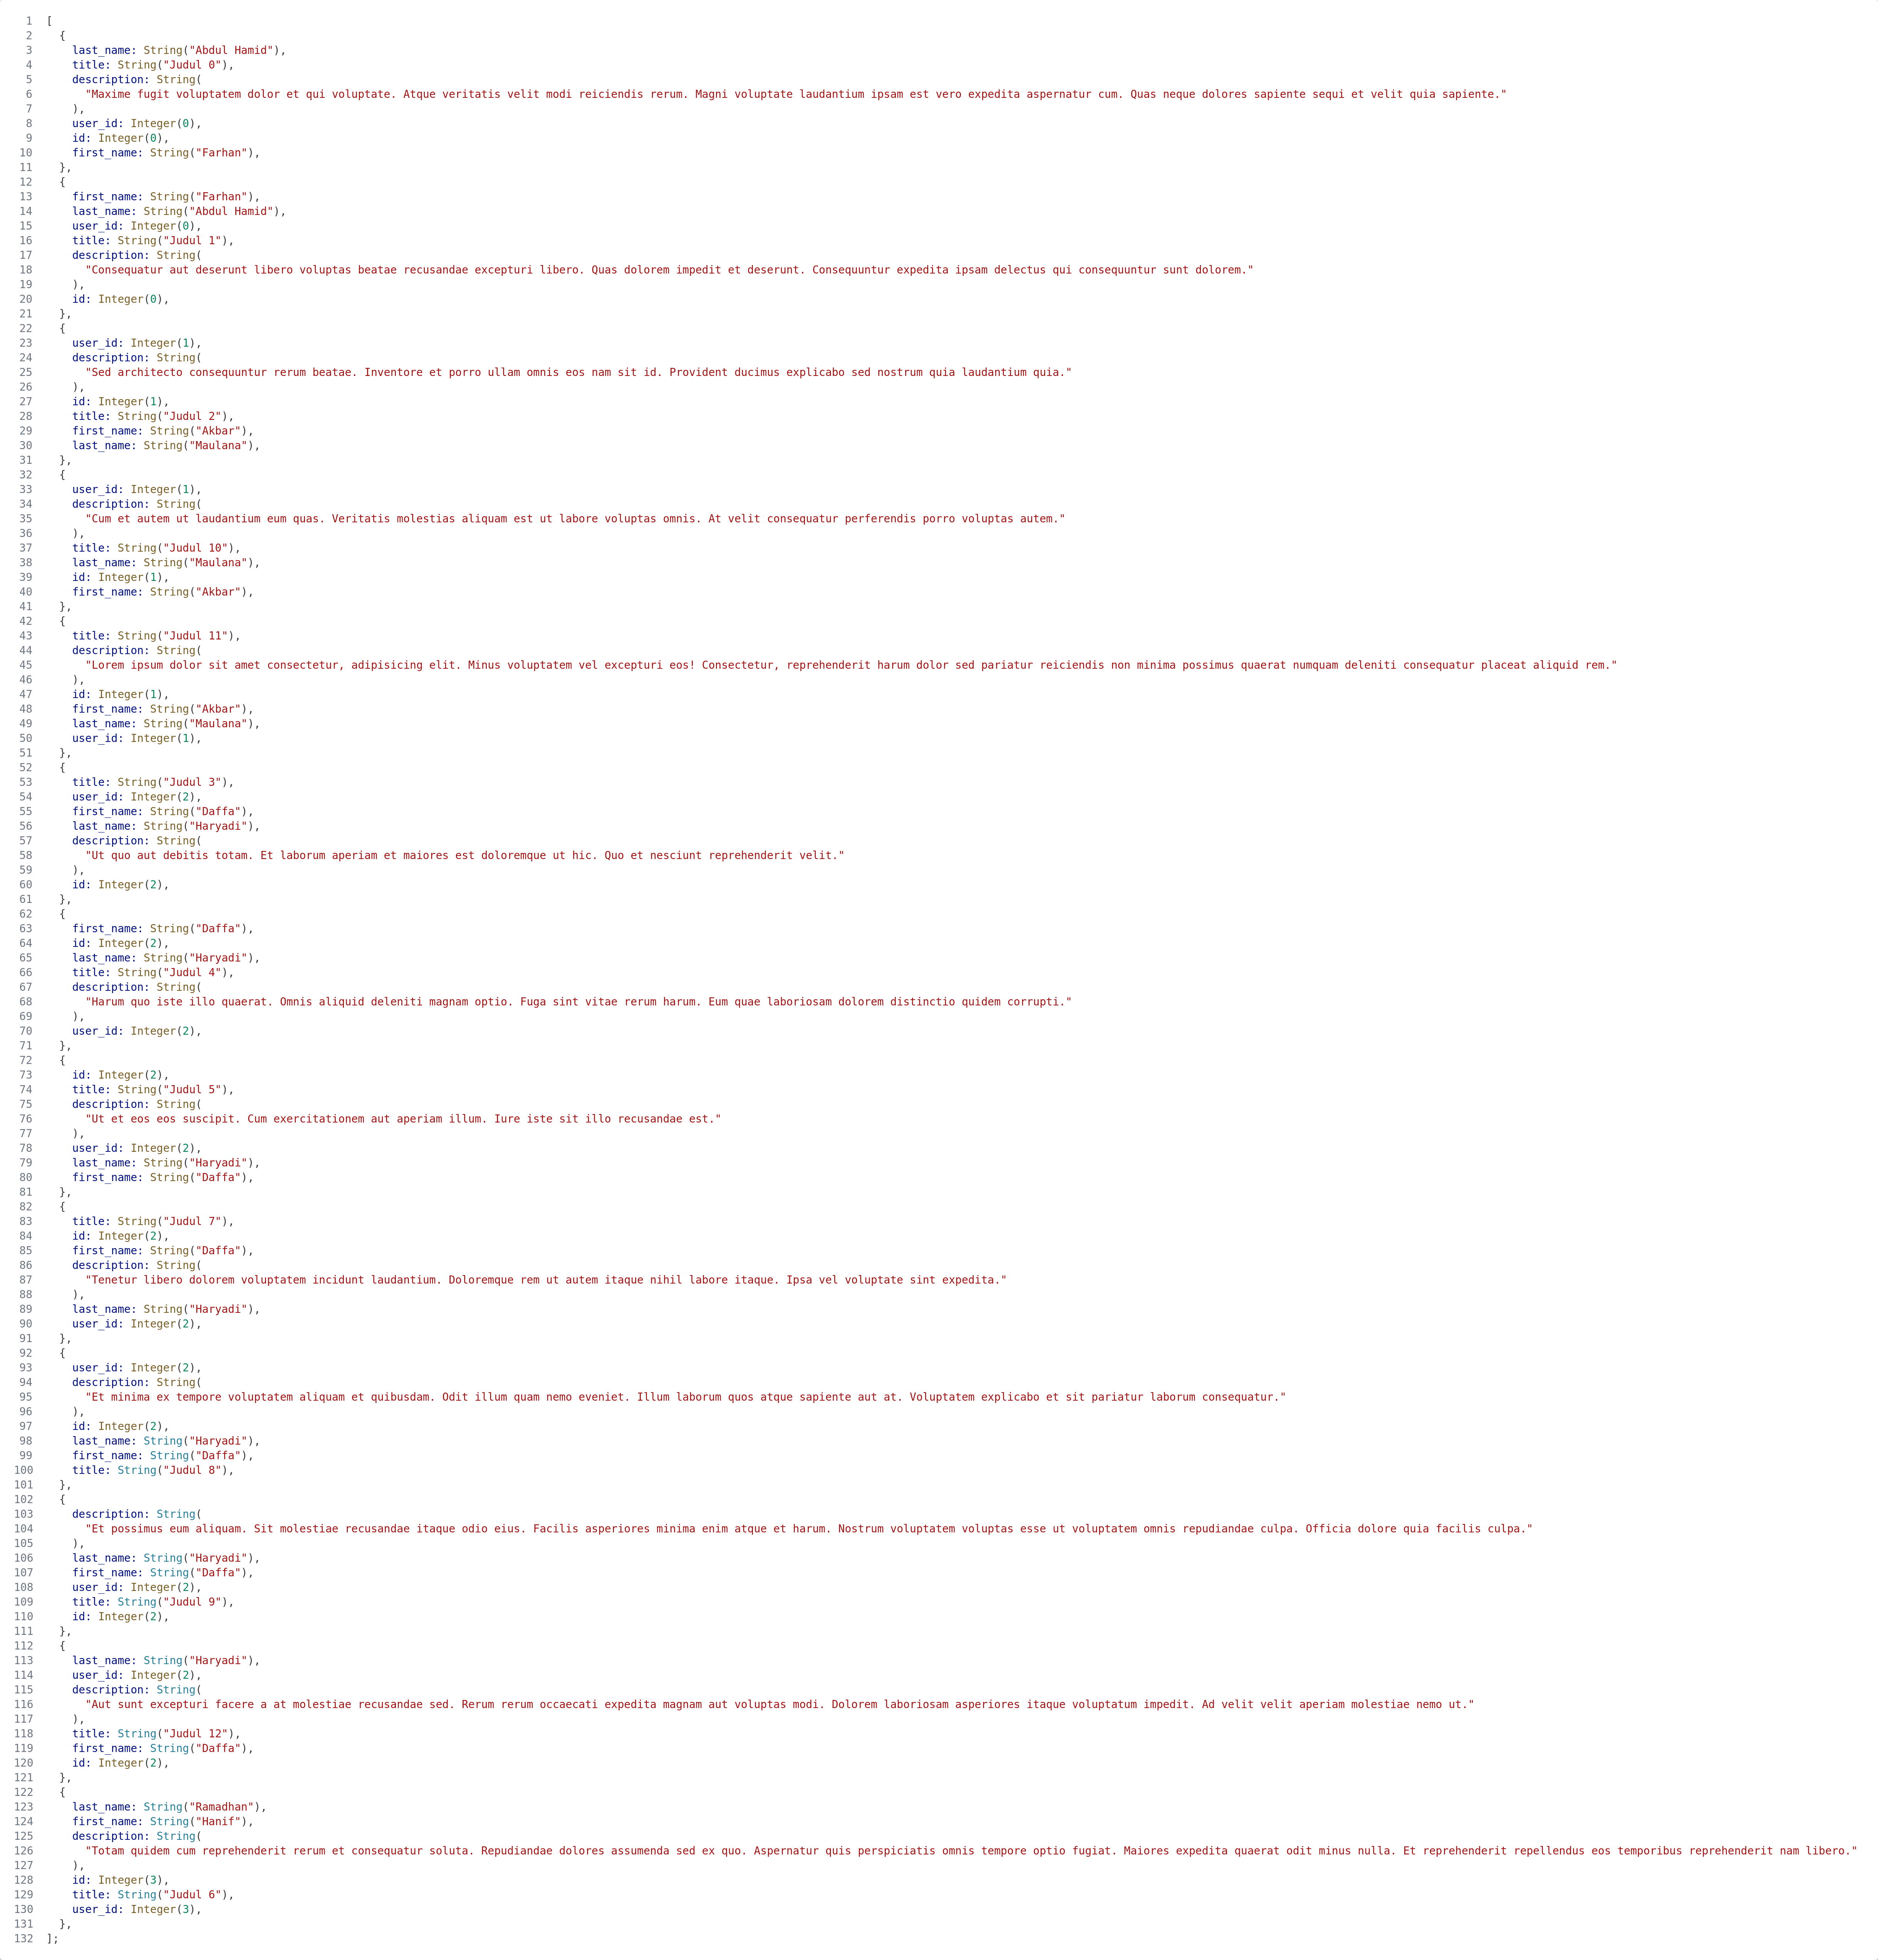
\includegraphics[width=0.9\textwidth]{gambar/bab4/test-join-data-inner-beautify.png}
  	\caption{Hasil data yang telah diformat menggunakan \emph{prettier} (\emph{Extension} VSCode pada Javascript)}
   \end{figure}
  \begin{figure}[H]
  	\centering{}
	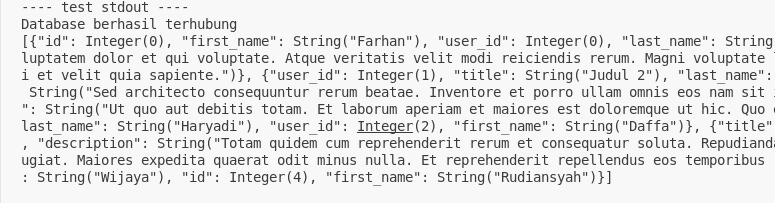
\includegraphics[width=0.6\textwidth]{gambar/bab4/test-join-data-left.png}
  	\caption{Informasi hasil \emph{left join}}
   \end{figure}
    \begin{figure}[H]
  	\centering{}
	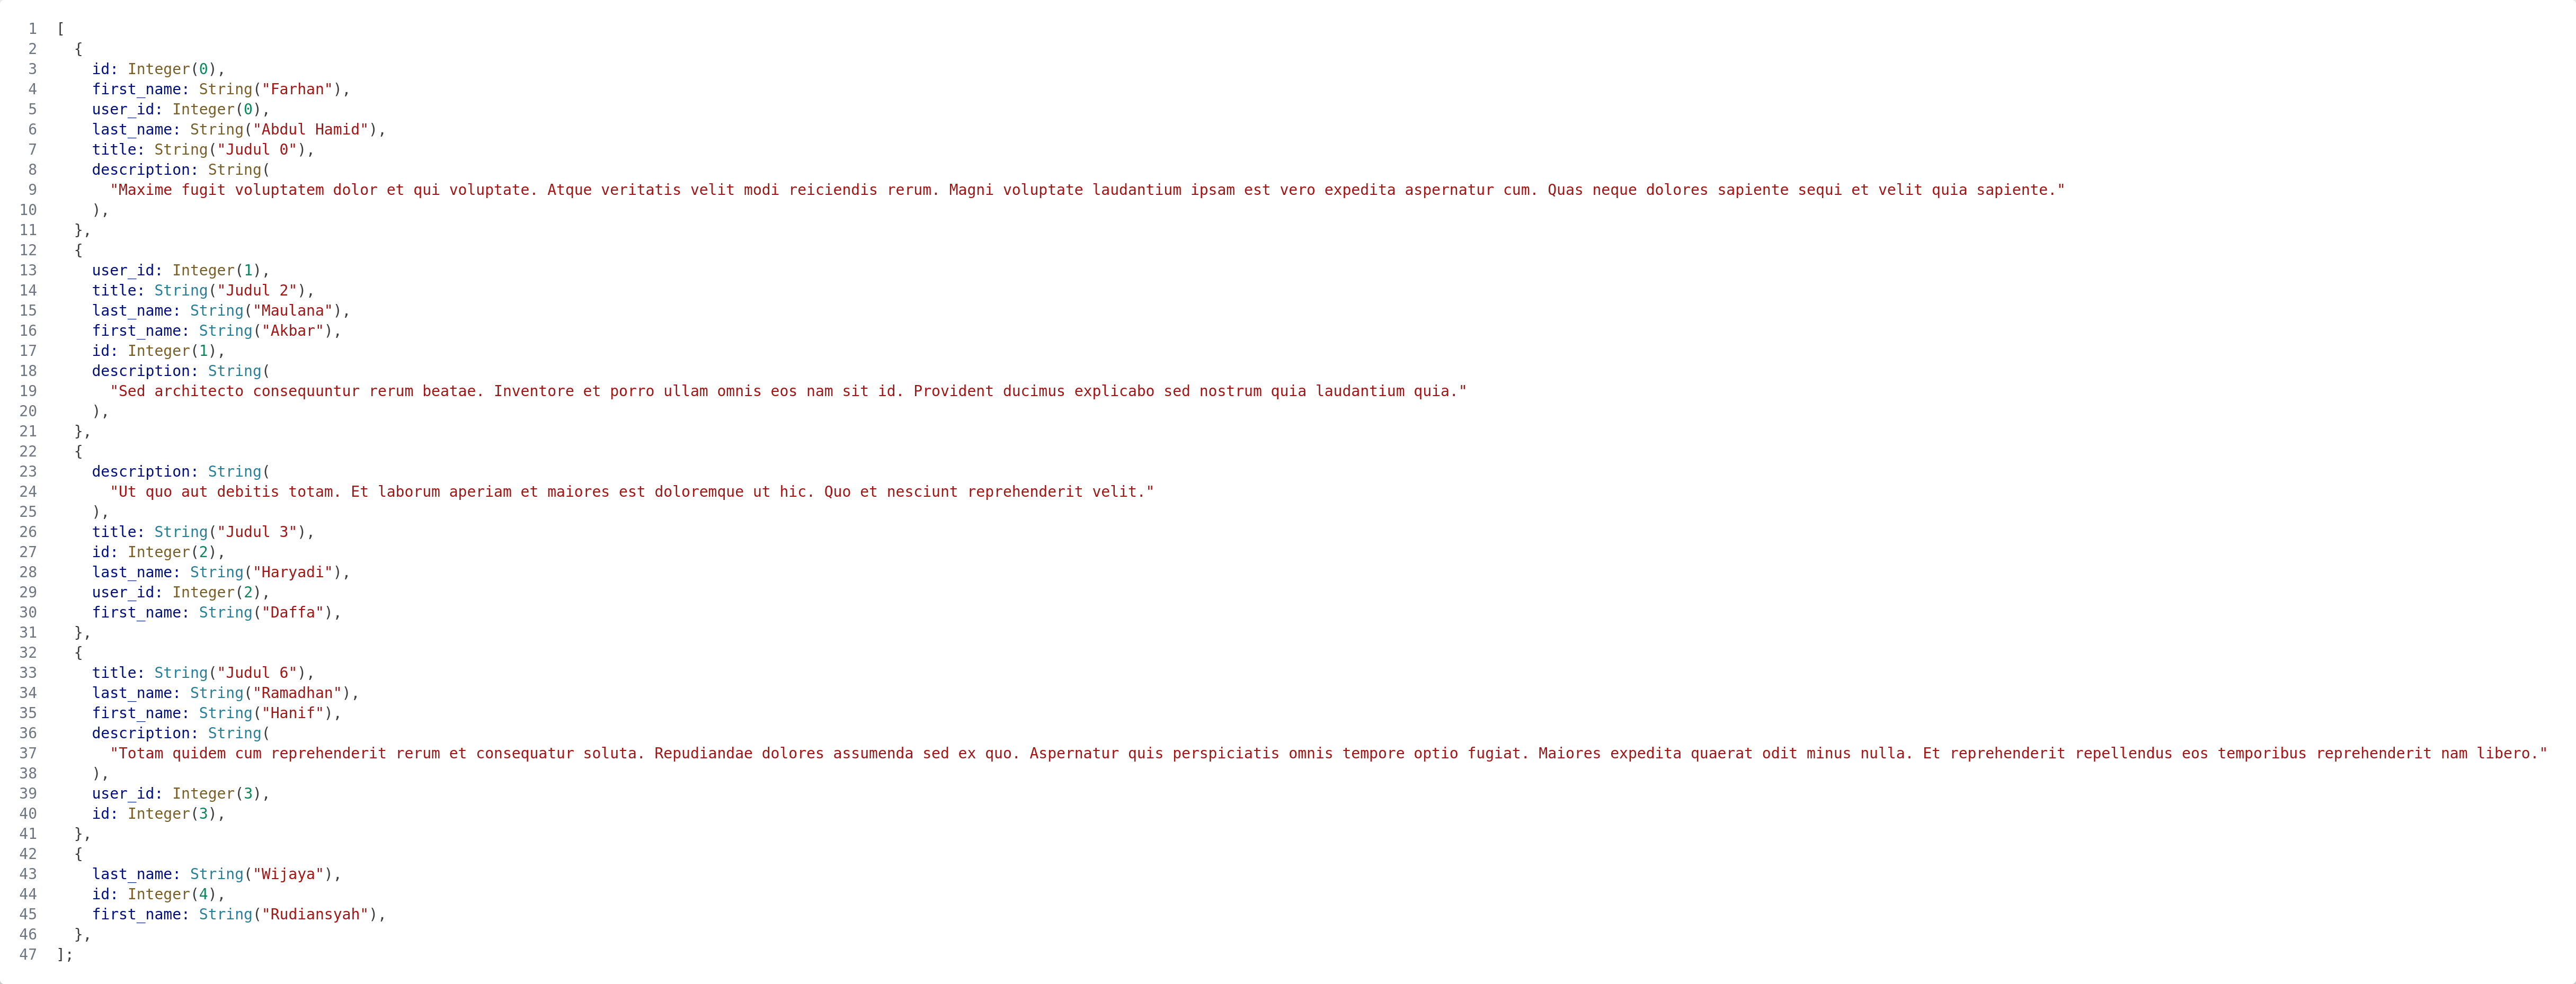
\includegraphics[width=0.9\textwidth]{gambar/bab4/test-join-data-left-beautify.png}
  	\caption{Hasil data yang telah diformat menggunakan \emph{prettier} (\emph{Extension} VSCode pada Javascript)}
   \end{figure}
  \begin{figure}[H]
  	\centering{}
	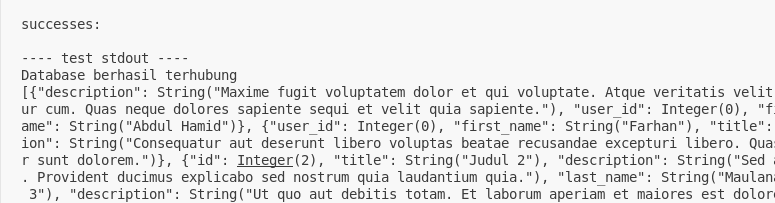
\includegraphics[width=0.6\textwidth]{gambar/bab4/test-join-data-right.png}
  	\caption{Informasi hasil \emph{right join}}
   \end{figure}
    \begin{figure}[H]
  	\centering{}
	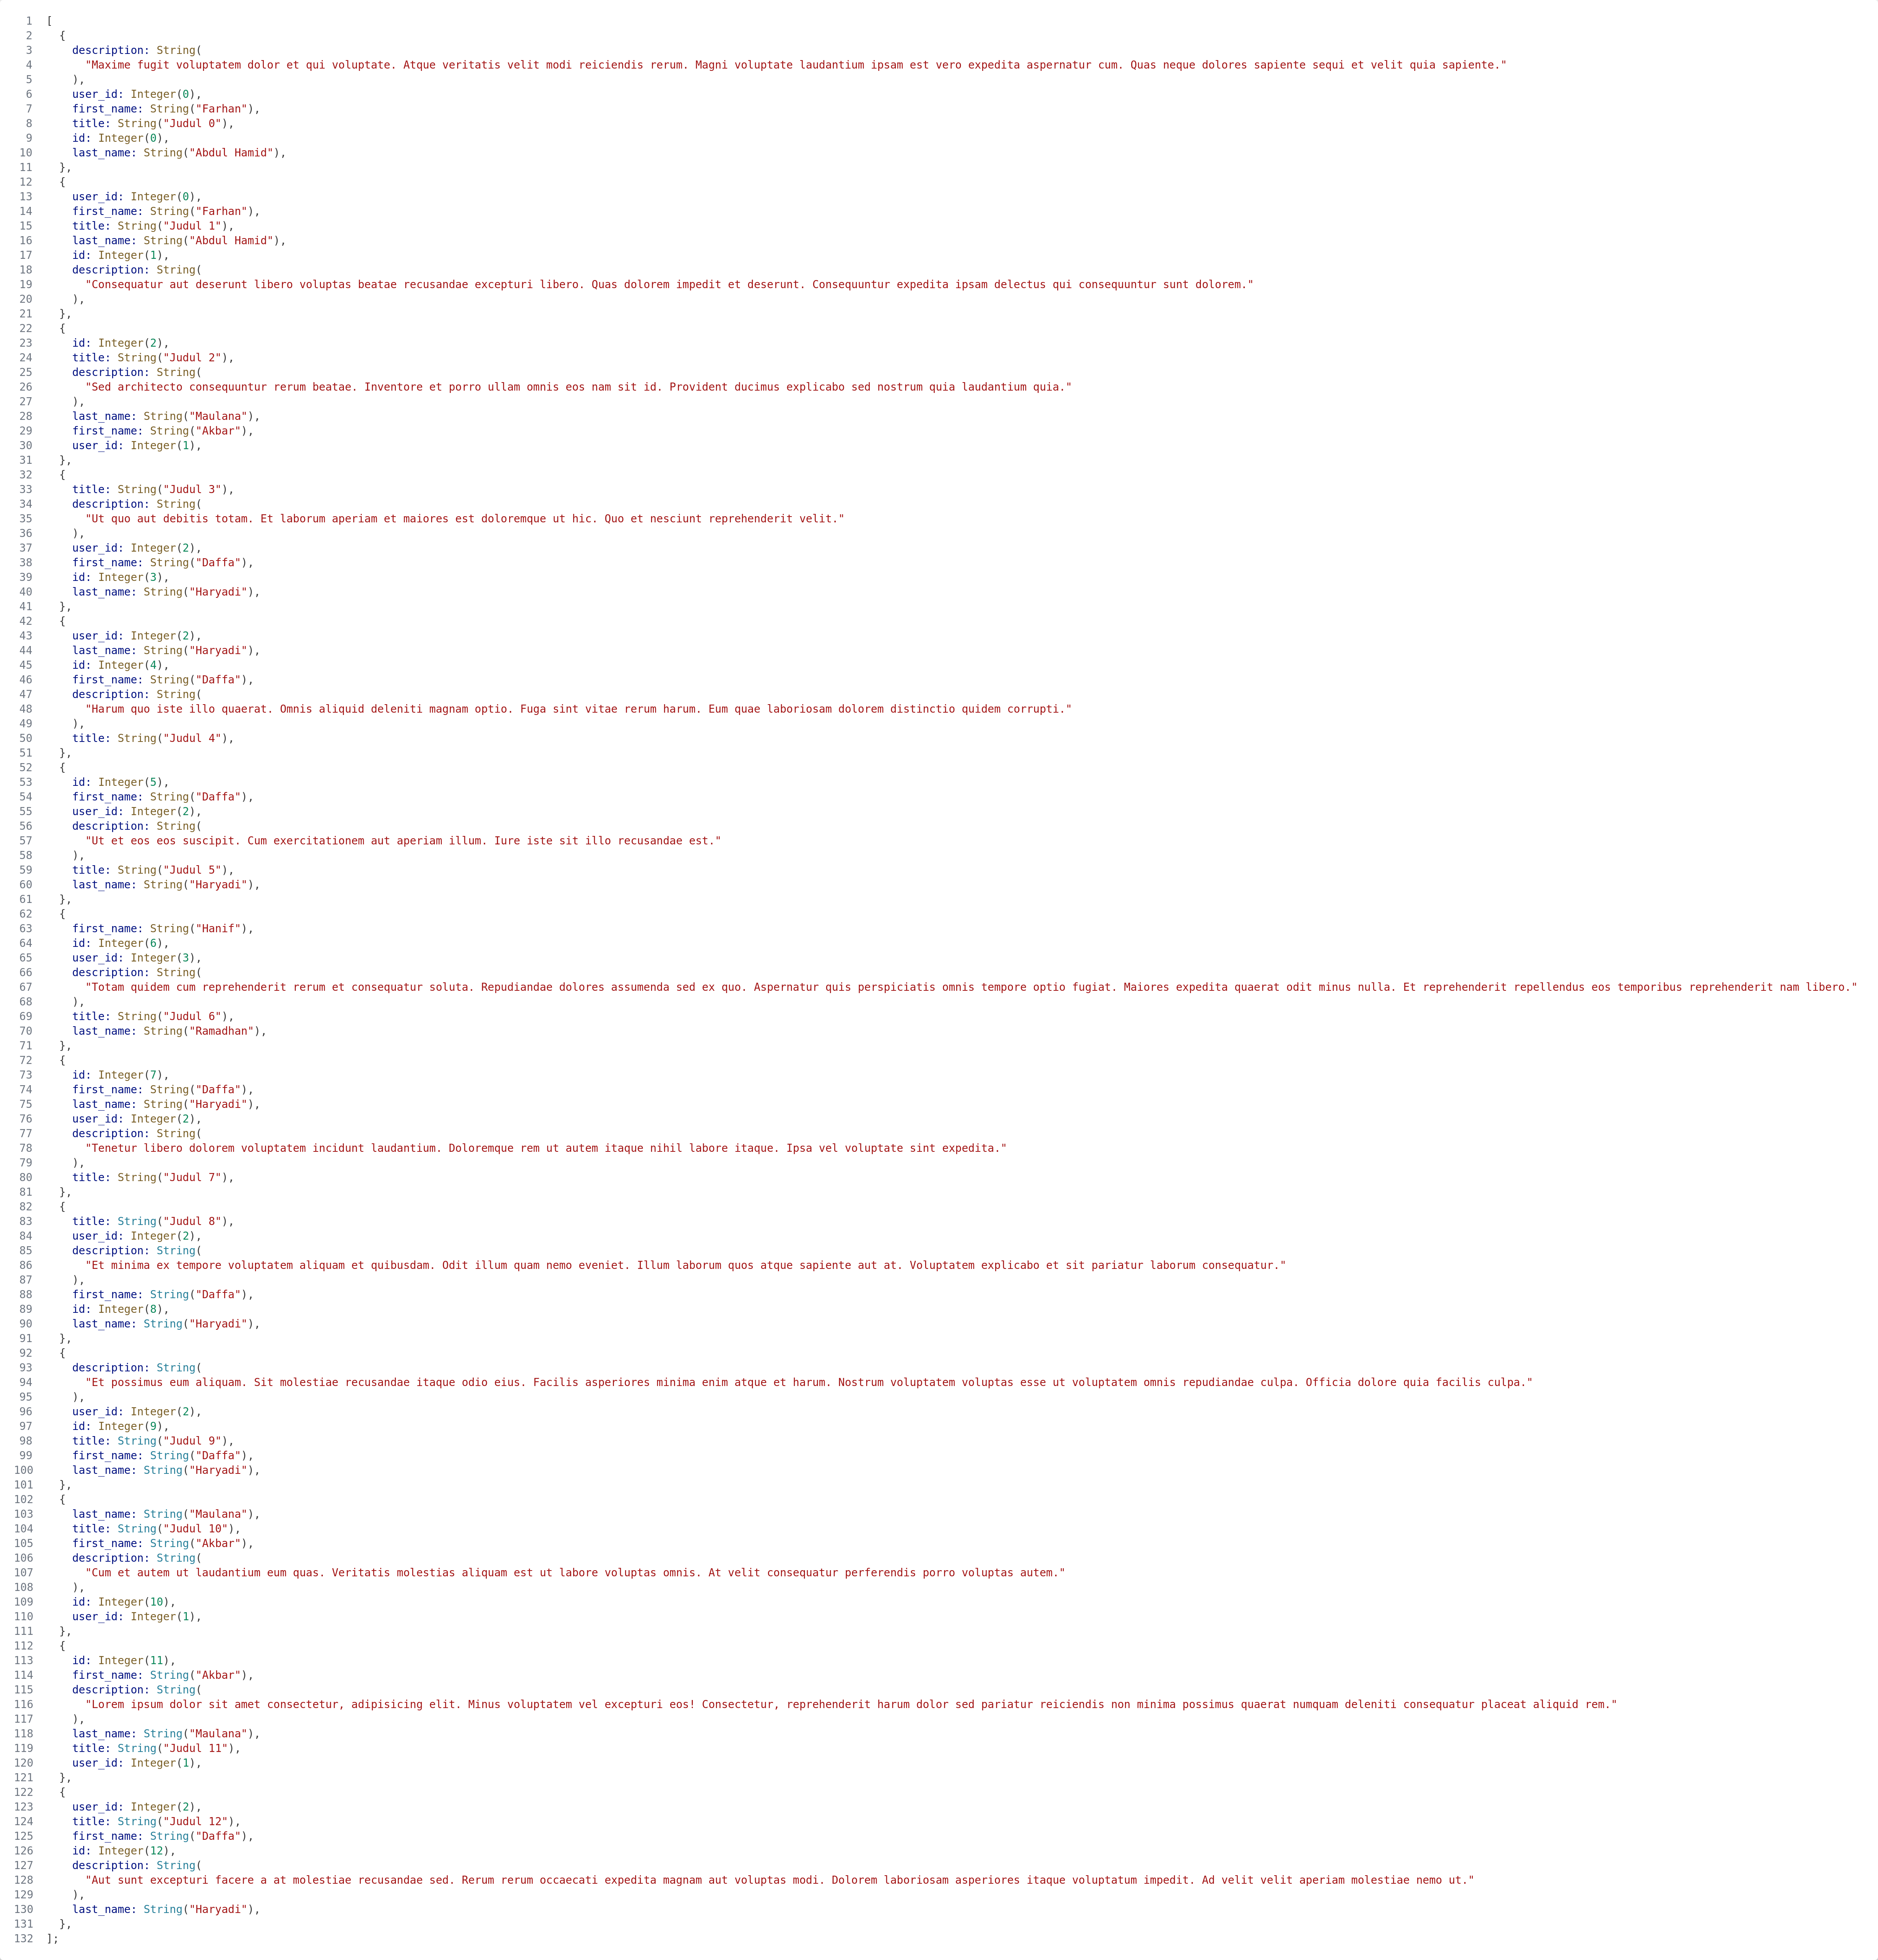
\includegraphics[width=0.9\textwidth]{gambar/bab4/test-join-data-right-beautify.png}
  	\caption{Hasil data yang telah diformat menggunakan \emph{prettier} (\emph{Extension} VSCode pada Javascript)}
   \end{figure}

	\item test\_delete\_data \\
  Pengujian \emph{method} delete data membutuhkan data mana saja yang akan dihapus, tentunya dengan menggunakan kolom tersedia di dalam tabel. Untuk kasus kali ini, data pada tabel users 
  akan dicoba untuk dihapus dengan ketentuan kolom first\_name yang memiliki value "Rudiansyah".
    \begin{figure}[H]
  	\centering{}
	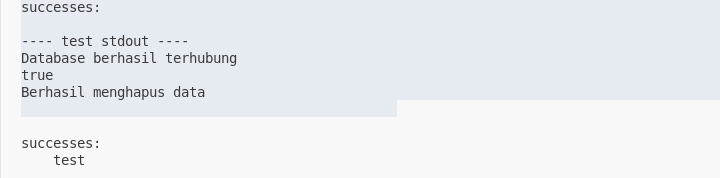
\includegraphics[width=0.6\textwidth]{gambar/bab4/test-delete-data.png}
  	\caption{Informasi hasil penghapusan data}
   \end{figure}
   \begin{figure}[H]
  	\centering{}
	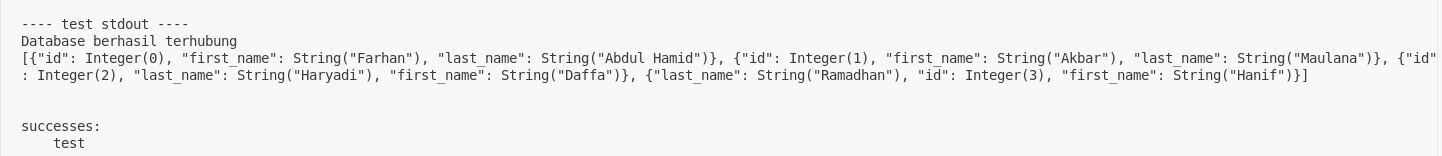
\includegraphics[width=0.6\textwidth]{gambar/bab4/test-hasil-delete.png}
  	\caption{Data tabel \emph{users} setelah value "Rudiansyah" dihapus}
   \end{figure}
  \begin{figure}[H]
  	\centering{}
	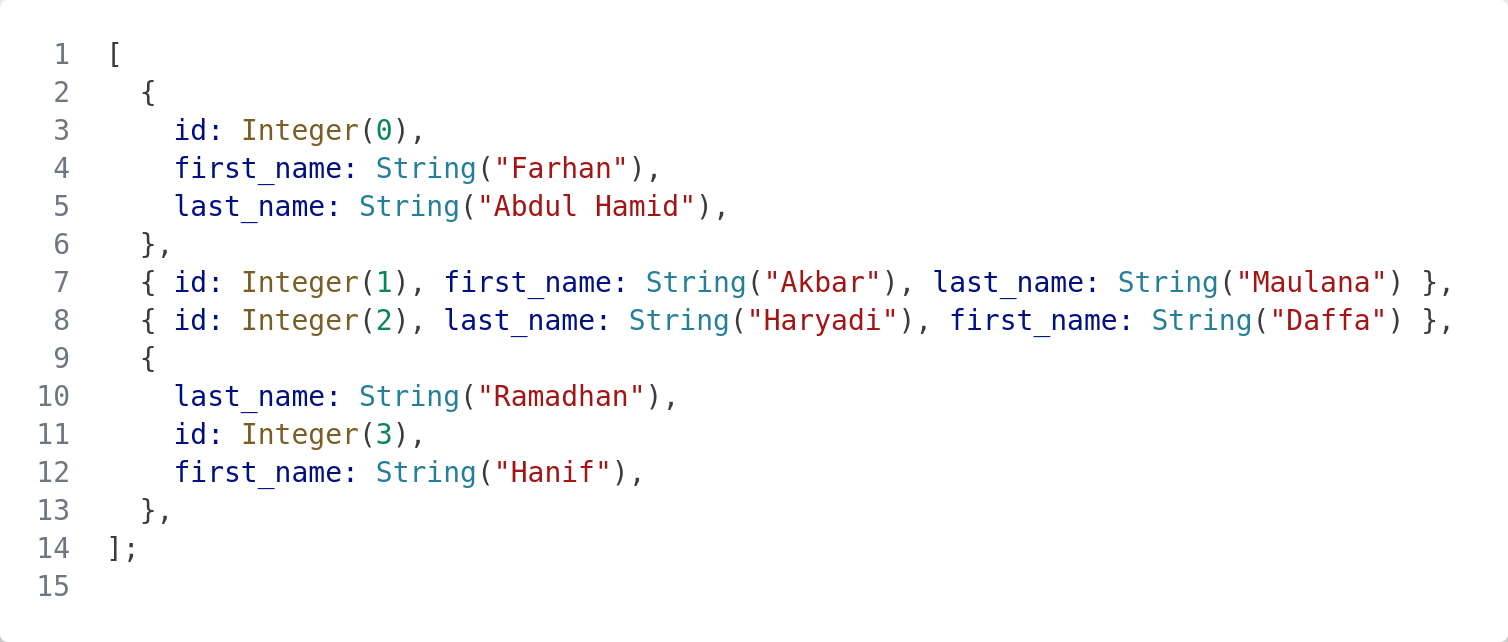
\includegraphics[width=0.9\textwidth]{gambar/bab4/test-hasil-delete-beautify.png}
  	\caption{Data tabel \emph{users} yang telah diformat menggunakan \emph{prettier} (\emph{Extension} \emph{Visual Studio Code} pada Javascript)}
   \end{figure}
\end{enumerate}

\emph{Return} pada setiap \emph{method} didalam \emph{DatabaseInterface} pada pengujian diatas tidak memengaruhi hasil pengujian karena 
untuk menampilkan data, pengujian menggunakan \emph{method} print dari struct yang telah dibuat. Lalu tidak semua \emph{method} yang ada pada \emph{class} \emph{TestDatabaseInterface} digunakan selama pengujian.

\subsection{Pengujian Eksternal}
Untuk melakukan pengujian eksternal diperlukan sebuah \emph{client} untuk memanggil \emph{interface} D-Bus yang telah dibuka. Pada pengujian kali ini, bahasa pemrograman python akan
digunakan beserta dengan library dbus-next. Pengujian akan dilakukan pada proses pembuatan, pengubahan dan penghapusan. Untuk pengambilan data masih belum bisa diuji
sebagaimana yang telah di kutip pada sub bab 4.1.11. Berikut adalah isian dari program \emph{client} menggunakan bahasa pemrograman python.

 \begin{figure}[H]
  	\centering{}
	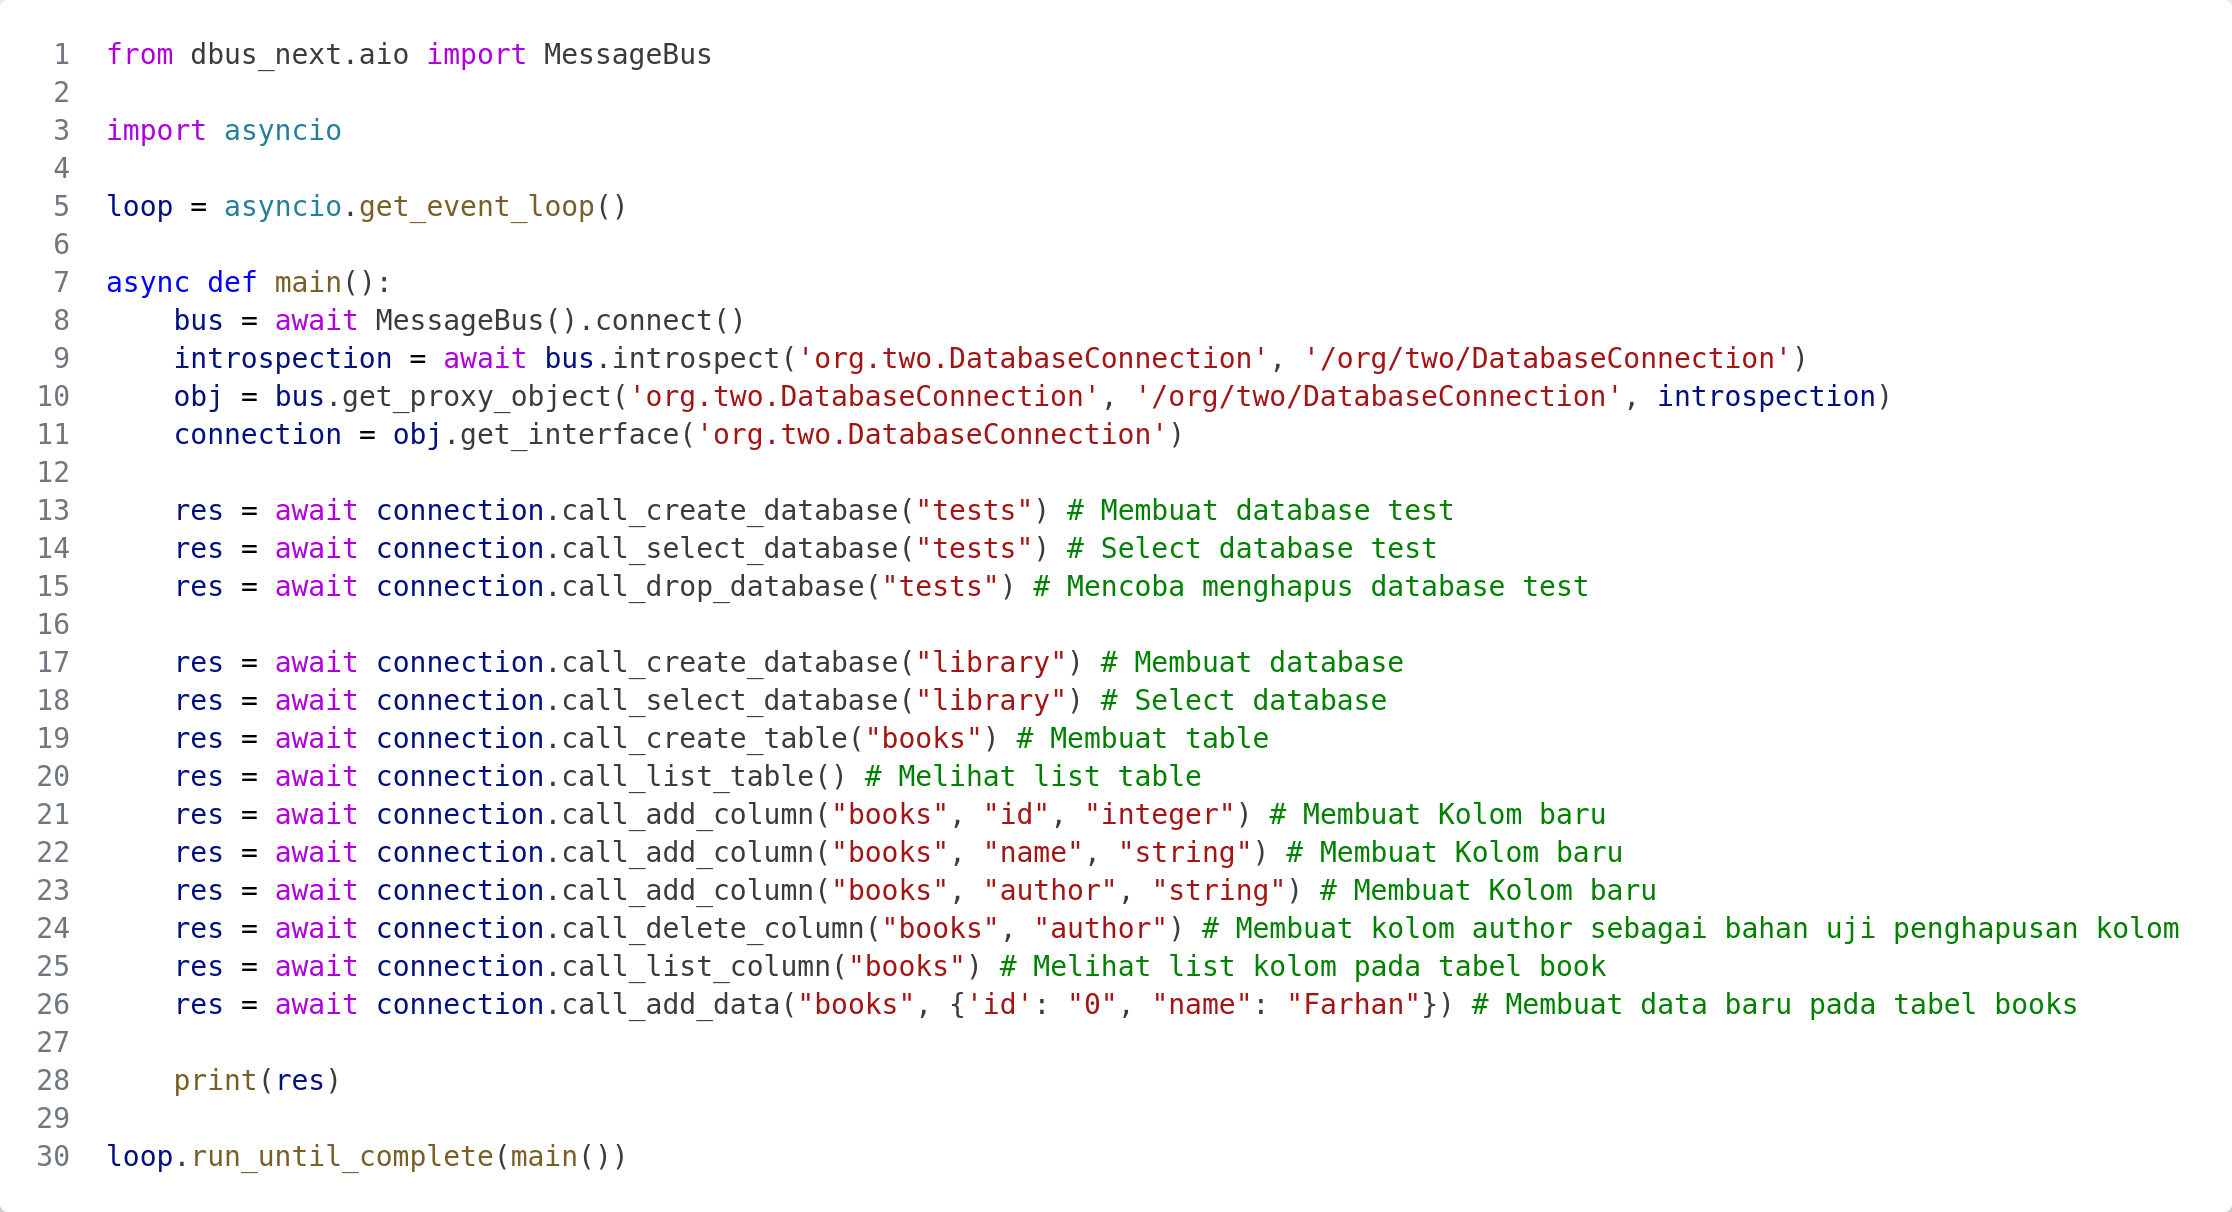
\includegraphics[width=0.8\textwidth]{gambar/bab4/uji-client.png}
  	\caption{Isi program pengujian \emph{client} dengan bahasa pemrograman Python}
   \end{figure}

    \begin{figure}[H]
  	\centering{}
	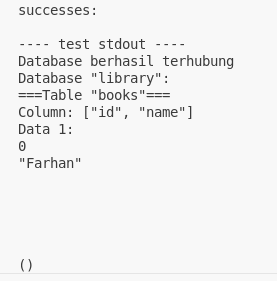
\includegraphics[width=0.6\textwidth]{gambar/bab4/hasil-uji-client.png}
  	\caption{Informasi hasil pengujian client}
   \end{figure}

Hasil dari pengujian \emph{client} dijalankan dengan \emph{method} print pada \emph{class} TestDatabaseInterface. \emph{Method} tersebut merupakan \emph{method} yang berguna untuk melihat keseluruhan
data yang tersimpan pada suatu \emph{database}.

\subsection{Pengujian Internal dengan Data Hasil \emph{Crawling}}
\emph{Database Engine} yang dikembangkan pada saat ini ditujukan untuk pengembangan sistem \emph{crawling} pada penelitian terakhir (\cite{ridho2024}). Karena alasan tersebut, pengujian menggunakan
data hasil \emph{crawling} pada penelitian sebelumnya (\cite{ridho2024}) akan dilakukan. Untuk pengujian tidak semua tabel akan digunakan, hanya 2 tabel hasil \emph{crawling} saja yaitu tabel bernama page\_information dan crawling.
Dalam tabel tersebut terdapat berbagai macam data, namun dikarenakan pada database saat ini hanya mendukung 2 tipe data yaitu \emph{string} dan \emph{integer}, maka untuk tipe data lain diluar dari 2 tipe data tersebut,
akan dirubah menjadi \emph{string}. Sebanyak 10 baris dari tabel page\_information akan digunakan, data tersebut dapat dilihat pada \emph{file} crawl\_information.json dalam \emph{folder} test-data.
Proses pengujian dilakukan dengan tahapan berikut:

\begin{enumerate}
	\item Membuat \emph{database}
	\item Membuat \emph{table} crawling dengan \emph{table} page\_information
	\item Melengkapi kolom pada \emph{table} crawling
	\item Mengisi data pada \emph{table} crawling
	\item Melengkapi kolom pada \emph{table} page\_information
	\item Mengisi data pada \emph{table} page\_information
	\item Menampilkan data yang telah terisi
\end{enumerate}

Dari hasil pengujian tersebut didapatkan bahwa, penyimpanan dan pengambilan dapat berjalan dengan baik. Namun hal tersebut hanya berlaku untuk huruf latin, untuk huruf-huruf bahasa lain seperti
bahasa china, jepang, arab dan lainnya masih belum dapat tersimpan dengan benar. Permasalahan ini harus ditelusuri lebih lanjut, namun ada kemungkinan bahwa penyimpanan 1 huruf selain huruf latin memiliki
ukuran yang berbeda dengan huruf latin. Berikut adalah contoh kesalahan penyimpanan dan penampilan data pada bahasa non latin:

\begin{figure}[H]
	\centering{}
	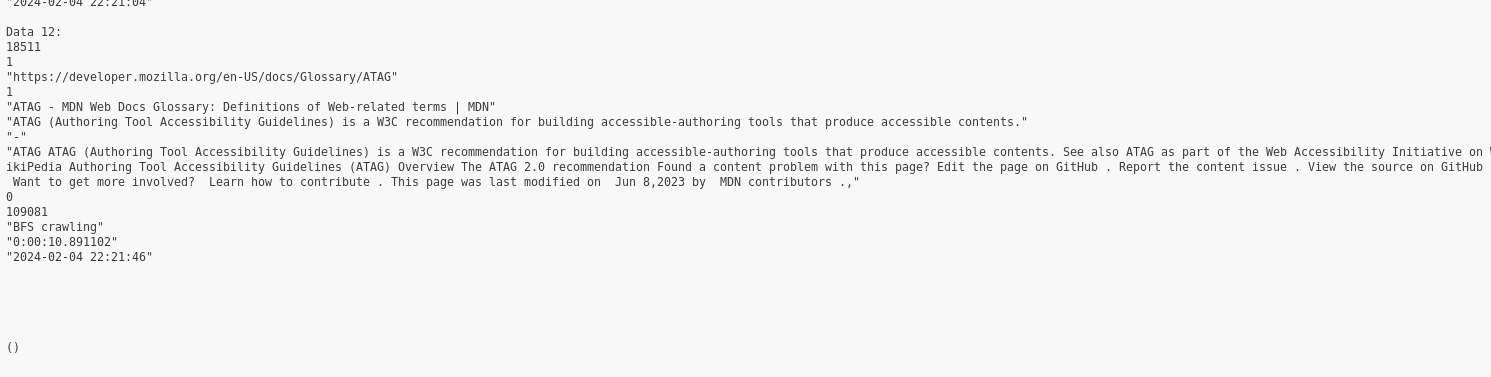
\includegraphics[width=0.95\textwidth]{gambar/bab4/hasil-pengujian-data-hasil-crawling.png}
	\caption{Informasi hasil pengujian data \emph{crawling}}
\end{figure}


\subsection{Hasil Implementasi}

Dari implementasi dan pengujian yang dilakukan pada sub bab sebelumnya, maka didapatkan sebuah \emph{database engine} baru yang dikembangkan dengan bahasa pemrograman Rust.
Pemrosesan yang terjadi dalam \emph{database engine} yang telah dibuat dapat dilihat pada setiap method-method yang telah dibuat. Pemrosesan tersebut mulai dari mengambil data,
menyimpan data, mengubah data dan menghapus data. Dari hasil pengujian pun dapat terlihat bahwa \emph{database} telah berhasil disimpan secara persisten dalam sebuah sebuah \emph{file}.
Tidak hanya itu, pola dan metode penyimpanan pun dapat terlihat dari urutan \emph{byte} yang disimpan pada \emph{file}. Dengan begitu pengembang ke depannya dapat mengubah dan menyesuaikan pola
pemrosesan data di dalam \emph{database} baru ini jika menemukan pola atau algoritma yang lebih efisien. Terlebih jika di kedepan hari \emph{database engine} ini akan di implementasikan pada 
\emph{distributed database}, maka algoritma sinkronisasi dapat di terapkan langsung di dalam \emph{class} Schema yang telah dibuat. Algoritma yang dipilih dikembalikan kepada pengembang \emph{database
engine} ini di kemudian hari.

Meski demikian masih terdapat banyak fitur dari \emph{database} ini yang belum berjalan dengan baik dan memerlukan penyempurnaan. Berikut adalah hal-hal yang dapat disempurnakan pada fitur \emph{database
engine} ini, yaitu:
\begin{enumerate}
	\item Melengkapi metode-metode eksternal untuk \emph{client} \\
  	Belum semua \emph{method} yang ada pada \emph{DatabaseInterface} terimplementasi pada \emph{DatabaseConnection}, sehingga membuat \emph{client} belum bisa menggunakan \emph{database engine} sepenuhnya.
	
	\item Memperbaiki return \emph{indexing} pada \emph{join} \\
	Dengan menerapkan \emph{indexing} yang ada pada \emph{database engine} saat ini, maka fitur \emph{join} tabel masih belum bisa berjalan dikarenakan tidak dapat mengembalikan data ke \emph{DatabaseConnection}.

	\item Menambahkan utilitas pada fitur \emph{join} \\
	Membuat fitur \emph{joining} untuk 3 tabel atau lebih, serta membuat constraint pada column yang menjadi key antar tabel.
	
	\item Melihat metadata pada column di \emph{database} \\
	Saat ini fitur untuk melihat list column, baru mengembalikan nama kolom saja dari tabel.

	\item Menambahkan metadata pada \emph{database} dan table \\
	Metadata yang umumnya ada pada fitur \emph{database management} seperti created\_at, increment, uniqueId dan lainnya.

	\item Menambahkan tipe data lain \\
	Menambahkan tipe data lain karena saat ini hanya bisa mendukung 2 tipe data yaitu String dan Integer.

	\item Pengubahan default value \\
	Menambahkan perubahan nilai default pada cell yang ada di \emph{database} agar nilai default dari sebuah cell dapat diubah.

	\item Membuat multi connection \\
	Saat ini koneksi yang dapat ditangani hanya 1 koneksi, jika digunakan untuk 2 koneksi \emph{client}, maka dikhawatirkan terdapat data yang tidak sinkron.

	\item Membuat kompatibilitas terhadap bahasa non latin \\
	Pada sistem \emph{database engine} yang berjalan saat ini, masih belum dapat menyimpan dan menampilkan data dengan bahasa non latin. Kemungkinan hal ini terjadi
	dikarenakan bahasa non latin memiliki jumlah \emph{byte} yang berbeda untuk satu karakter dibanding dengan satu karakter huruf latin.

	\item Pembuatan \emph{folder} \emph{schema} dan \emph{index} secara otomatis  \\
	Setelah melakukan proses \emph{build}, jika hasil \emph{build database engine} ingin dikirim ke perangkat lain, maka untuk saat ini \emph{folder} \emph{schema} dan \emph{folder}
	\emph{index} harus dibuat manual. 

	\item Memperbaiki dan menyempurnakan penanganan \emph{error} \\
  	Error yang ada pada saat ini hanya bisa dilihat dari server dan belum di handle dengan baik pada \emph{client}. Hal ini dapat menyebabkan \emph{client} tidak tau pasti penyebab error.
	Terdapat beberapa \emph{error} lain seperti saat hendak melakukan pembuatan database tanpa adanya \emph{folder} \emph{schema} dan \emph{index}. Jika tidak ada kedua \emph{folder} tersebut 
	maka database tidak terbuat, dan langsung memunculkan pesan "\emph{Database Created!}". Tentunya pesan yang disampaikan
	tidaklah sesuai, hal ini dikarenakan penanganan \emph{error} di \emph{Database Interface} masih belum baik. Tidak menutupi kemungkinan bahwa masih terdapat
	penanganan error lain yang harus ditingkatkan seperti jika path dari D-Bus sudah dipakai oleh sistem lain dan lainnya.

\end{enumerate}

\section{Sumber dan Orisinalitas \emph{code}}
Dalam pengembangan \emph{database engine}, berbagai macam sumber \emph{code} pihak lain digunakan sebagai referensi. Sumber-sumber tersebut dari beberapa \emph{website} 
serta dokumentasi langsung bahasa pemrograman dan \emph{library} yang digunakan selama pengembangan. Salah satu bagian penting pada pengembangan yang didapatkan dari 
referensi lain adalah proses perubahan dari sebuah data menjadi bentuk byte serta mengembalikannya dalam bahasa pemrograman rust. Hasil akhir dari \emph{source code} dapat dilihat pada \emph{link} berikut.

\begin{center}
	\href{https://github.com/arhandev11/database-engine}{https://github.com/arhandev11/database-engine}
\end{center}

Selain itu, sumber untuk melakukan penerapan metode \emph{waterfall} juga digunakan sebagai pembanding dengan penulisan yang dibuat. Hal ini dilakukan karena selama 
pengembangan berlangsung masih belum menggunakan metode \emph{waterfall}. Sumber lain seperti dokumentasi resmi postgresql dan lainnya digunakan sebagai
sumber pengetahuan dan pertimbangan dalam pengembangan \emph{database engine}. Penggunaan \emph{Artificial Intelligence} dengan model \emph{Gemini 2.5 pro} dan \emph{Chatgpt (Versi o4-mini-high, 4.1 dan 5)} juga
digunakan dalam memahami isi \emph{paper} serta dalam membantu membuat penulisan dan \emph{formatting} menggunakan \emph{latex}.

% Baris ini digunakan untuk membantu dalam melakukan sitasi
% Karena diapit dengan comment, maka baris ini akan diabaikan
% oleh compiler LaTeX.
\begin{comment}
\bibliography{daftar-pustaka}
\end{comment}
